\documentclass[noframe,oneside]{ncuthesisCJK}
\usepackage{makeidx}             % for index
\usepackage{layout}
\usepackage[]{todonotes}

\usepackage{cite}

\usepackage{graphicx}
\usepackage{amsmath}
\usepackage{amssymb}
\usepackage{amsfonts}
\usepackage{epsfig}
\usepackage{subcaption}
\usepackage{indentfirst}
\usepackage{color}
%\usepackage{txfonts}
%%%%%%%%%%
\usepackage{esvect}
\usepackage{epstopdf}

%\usepackage{algorithmic}
\usepackage[normalem]{ulem}
\usepackage{mathtools}
%\usepackage{txfonts}
\captionsetup{compatibility=false}
\graphicspath{{./figures/}}
%\newtheorem{definition}{Definition}
%\newtheorem{lemma}{Lemma}
\makeatletter
\renewcommand*{\@opargbegintheorem}[3]{\trivlist
      \item[\hskip \labelsep{\bfseries #1\ #2}] \textbf{(#3)}\ \itshape}
\makeatother
\usepackage{graphicx}
\usepackage{CJKutf8}
\usepackage{amsmath}
\usepackage{amssymb}
\usepackage{amsthm}
\usepackage{amsfonts}
\usepackage{epsfig}
\usepackage{subcaption}
\usepackage{indentfirst}
\usepackage{xcolor}
\usepackage{esvect}
\usepackage{epstopdf}
\usepackage[normalem]{ulem}
\usepackage{lipsum}
\usepackage{subcaption}
%\usepackage{gensymb}

\usepackage{multirow}
\usepackage{float}
\usepackage[ruled,lined]{algorithm2e}
\usepackage{algcompatible}

\usepackage[normalem]{ulem}
\usepackage{tabularx}
\usepackage{float}
\usepackage{caption,subcaption}
\captionsetup{compatibility=false}
\SetKwInOut{Parameter}{Parameters}
\SetKwInOut{INIT}{Initialization}
\usepackage{makecell}
\usepackage{afterpage}


\dept{數學研究所}
\degree{碩士}
\title{Multi-robot Search in 3D Environments using Submodularity with Matroid Intersection Constraints}
\subtitle{}
\author{李晏碩}
\authoren{Yan-Shuo, Li}
\mprof{曾國師}
\mprofen{Kuo-Shih, Tseng}
\sprof{}
\degreedate{中~華~民~國~一百一十三~年~六~月}
\copyyear{2024}
\def\XeLaTeX{Xe\LaTeX}   % Only in CJK
\def\scalefactor{1}        % define a new command
\newcommand\insertfig[3]{
\renewcommand\scalefactor{#3}
\begin{figure}[!hbt]
\centering
\includegraphics[scale=\scalefactor]{#1}
\caption{#2}
\label{Fig:#1}
\end{figure}
}
\newtheorem{theorem}{Theorem}[chapter]
\newtheorem{pr} {作業}[chapter]
\newtheorem{pf} {證明}[chapter]
\newtheorem{algo}{演算法}[chapter]
\newtheorem{definition}{Definition}
\newtheorem{lemma}{Lemma}
\newtheorem{corollary}{Corollary}[theorem]

% what follows are for watermark, mark these out if no need
\usepackage{background}
\SetBgContents{
\includegraphics{NCUlogo}} % need a watermark
\SetBgAngle{0}                                           % rotate
\SetBgColor{black!40}                                 % color
\SetBgScale{1.5}                                          % scale
\SetBgHshift{100}                                        % location x=0 for center
\SetBgVshift{230}                                        % location y=0 for center
% end of watermark codes
             % 自訂巨集多 收起來
                                            % 自訂巨集少 直接寫出

%\includeonly{chapter2}      % 單獨編譯此檔
\makeindex                           % 告訴\LaTeX要做索引
\begin{document}                 % 宣告結束   本文開始
\begin{CJK}{UTF8}{bkai}   %----------------------
\CJKhorz
\fontsize{14pt}{20pt}\selectfont % 可調間距以便閱讀%
\pagenumbering{alph}               % to cheat latex
\maketitle                       % 論文封面
\setboolean{printcopyright}{true}
\maketitle                       % 書名面
\cleardoublepage
\addtocontents{toc}{~\hfill\textbf{Page}\par}
%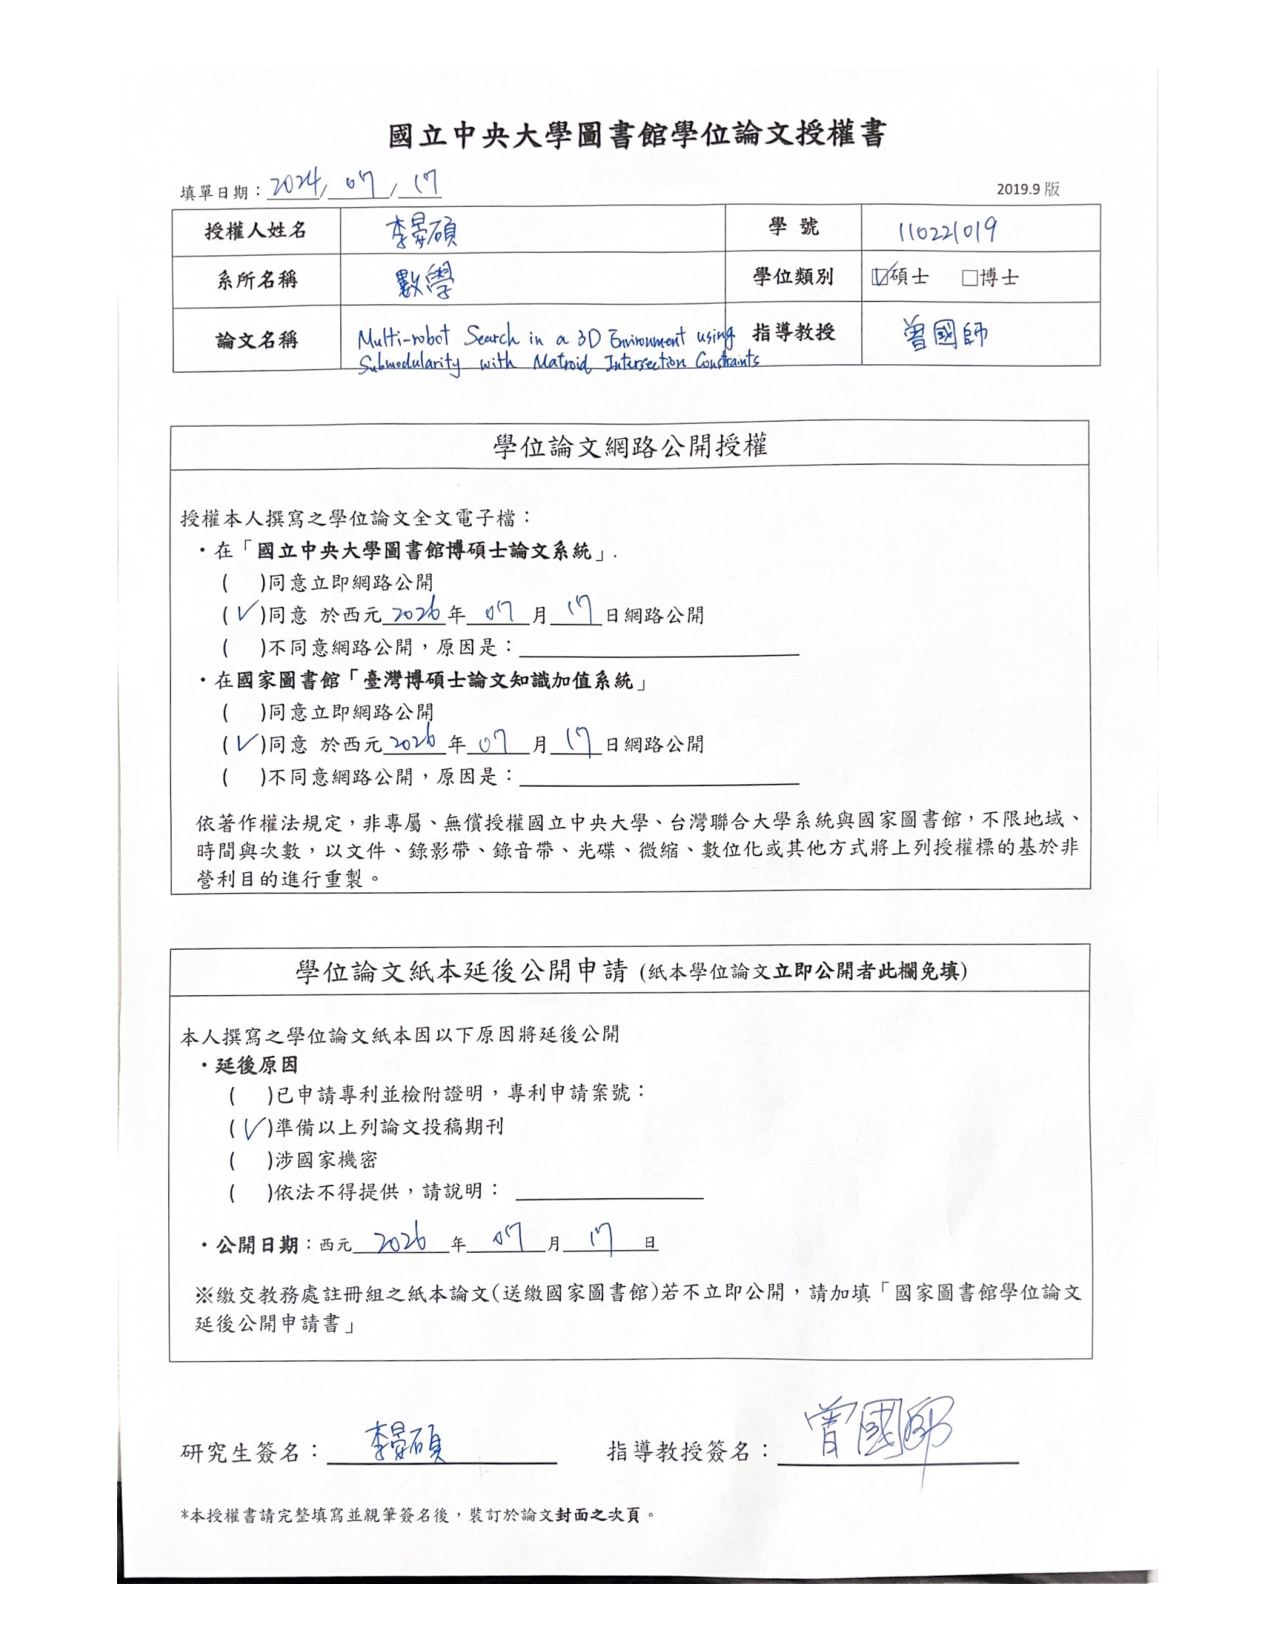
\includepdf[pages=-,scale=0.9]{4.pdf}
%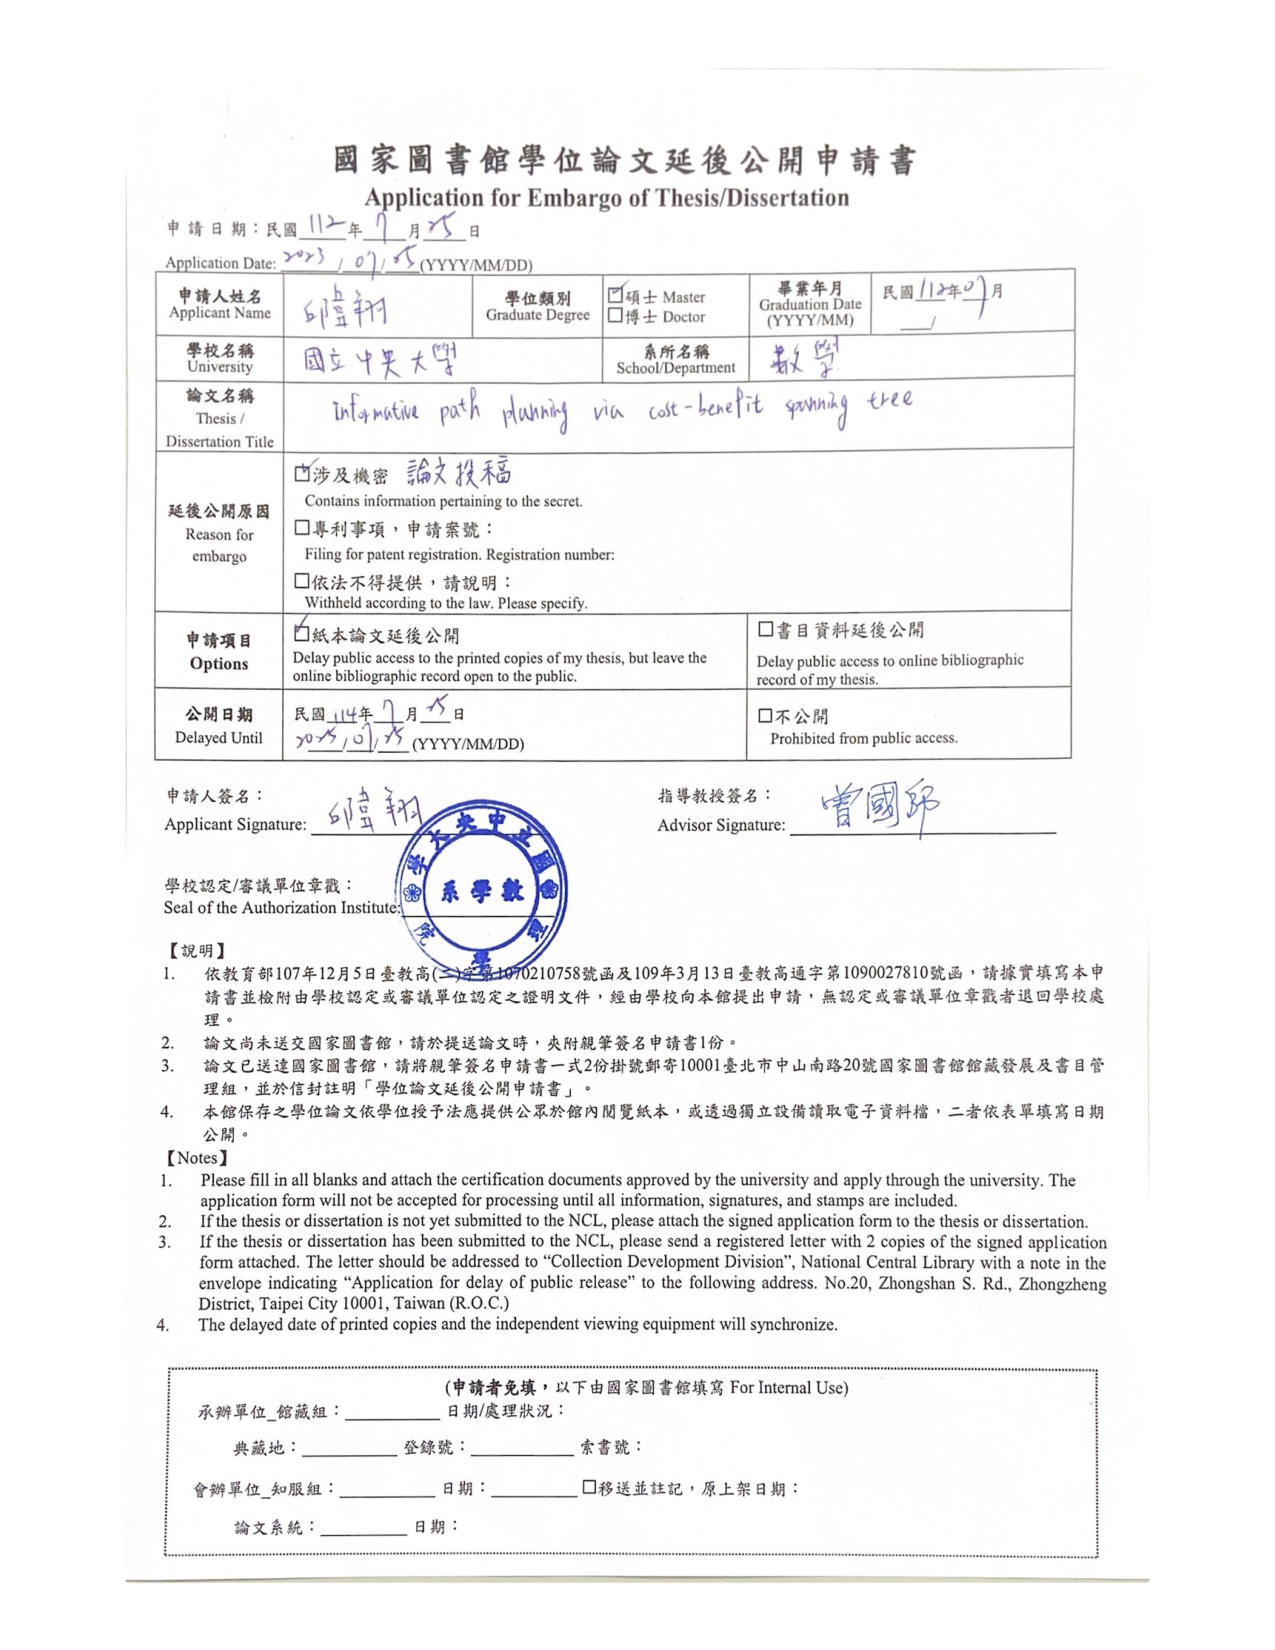
\includepdf[pages=-,scale=0.9]{3.pdf}
%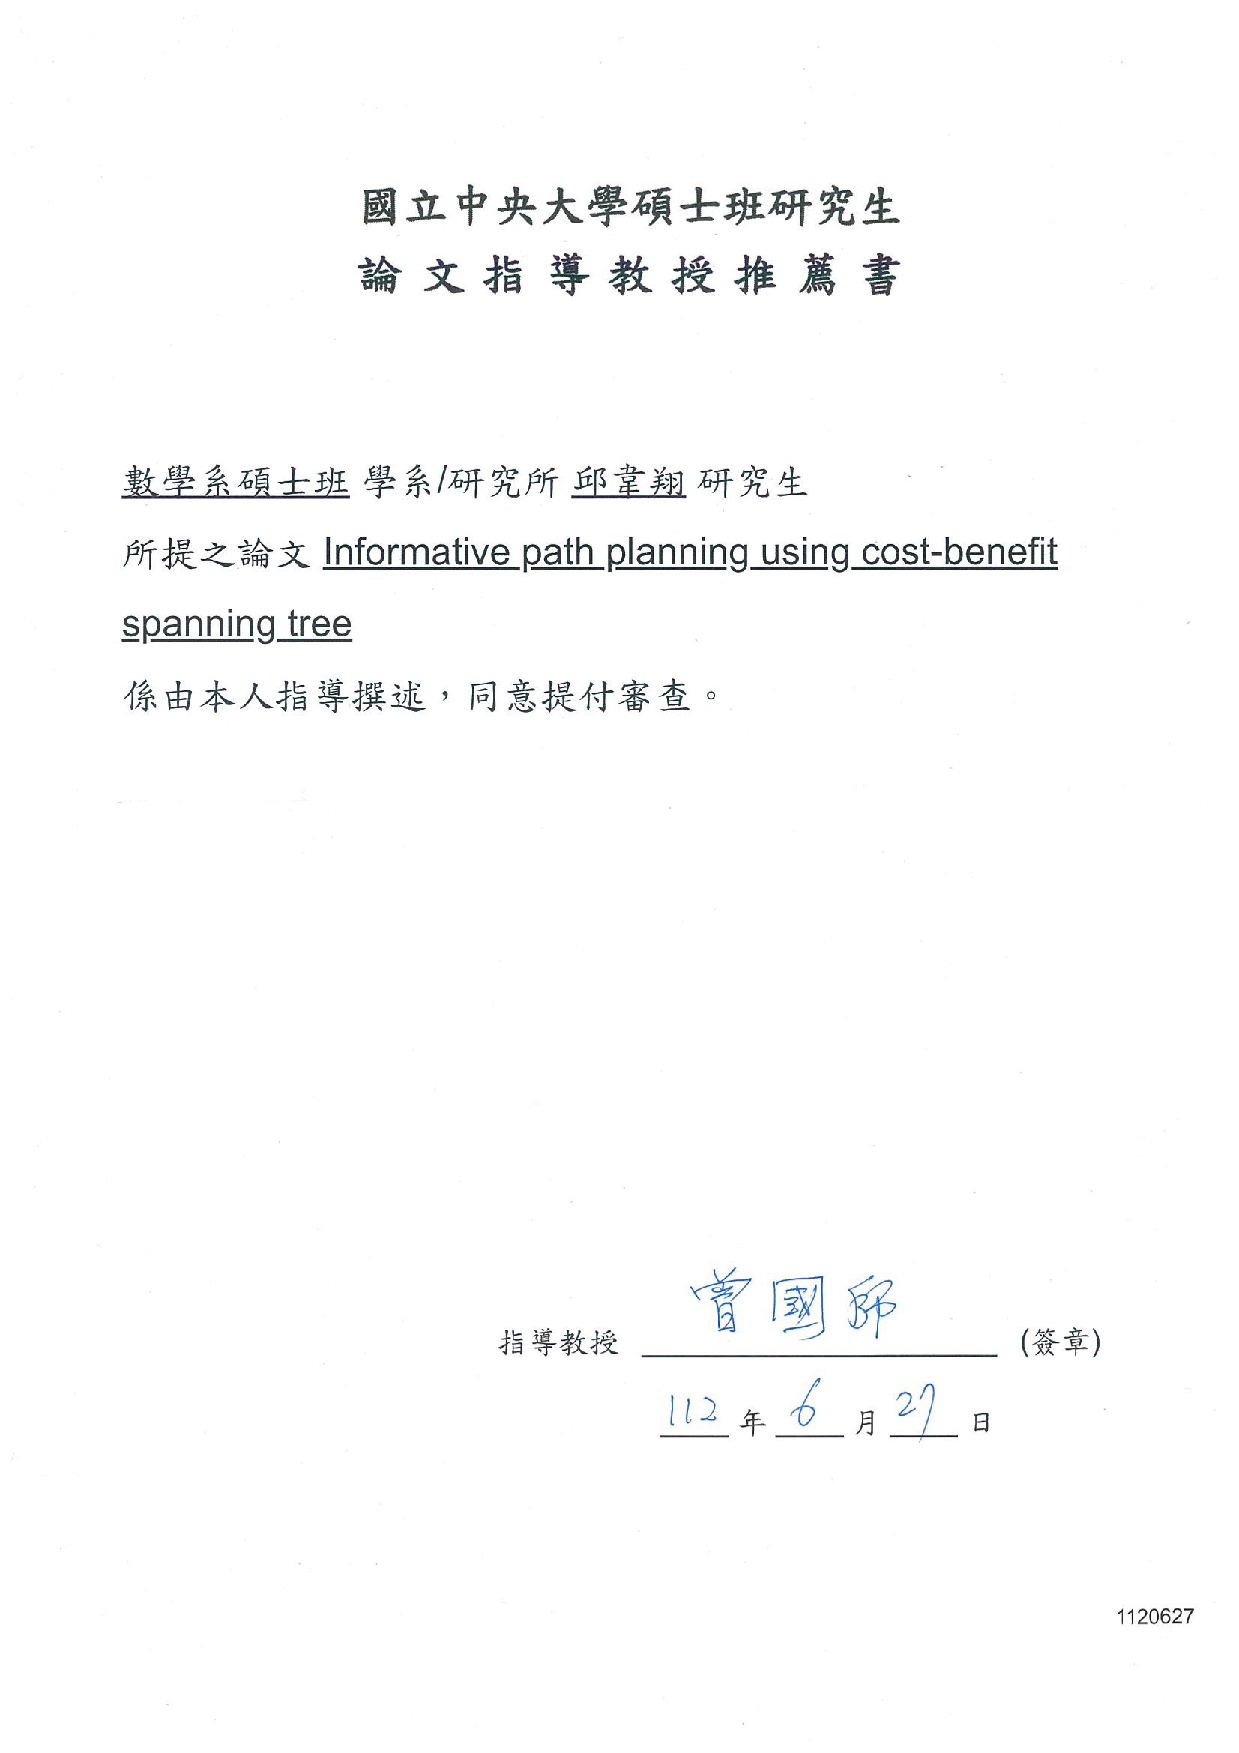
\includepdf[pages=-,scale=0.9]{1.pdf} % 插入其他表格
%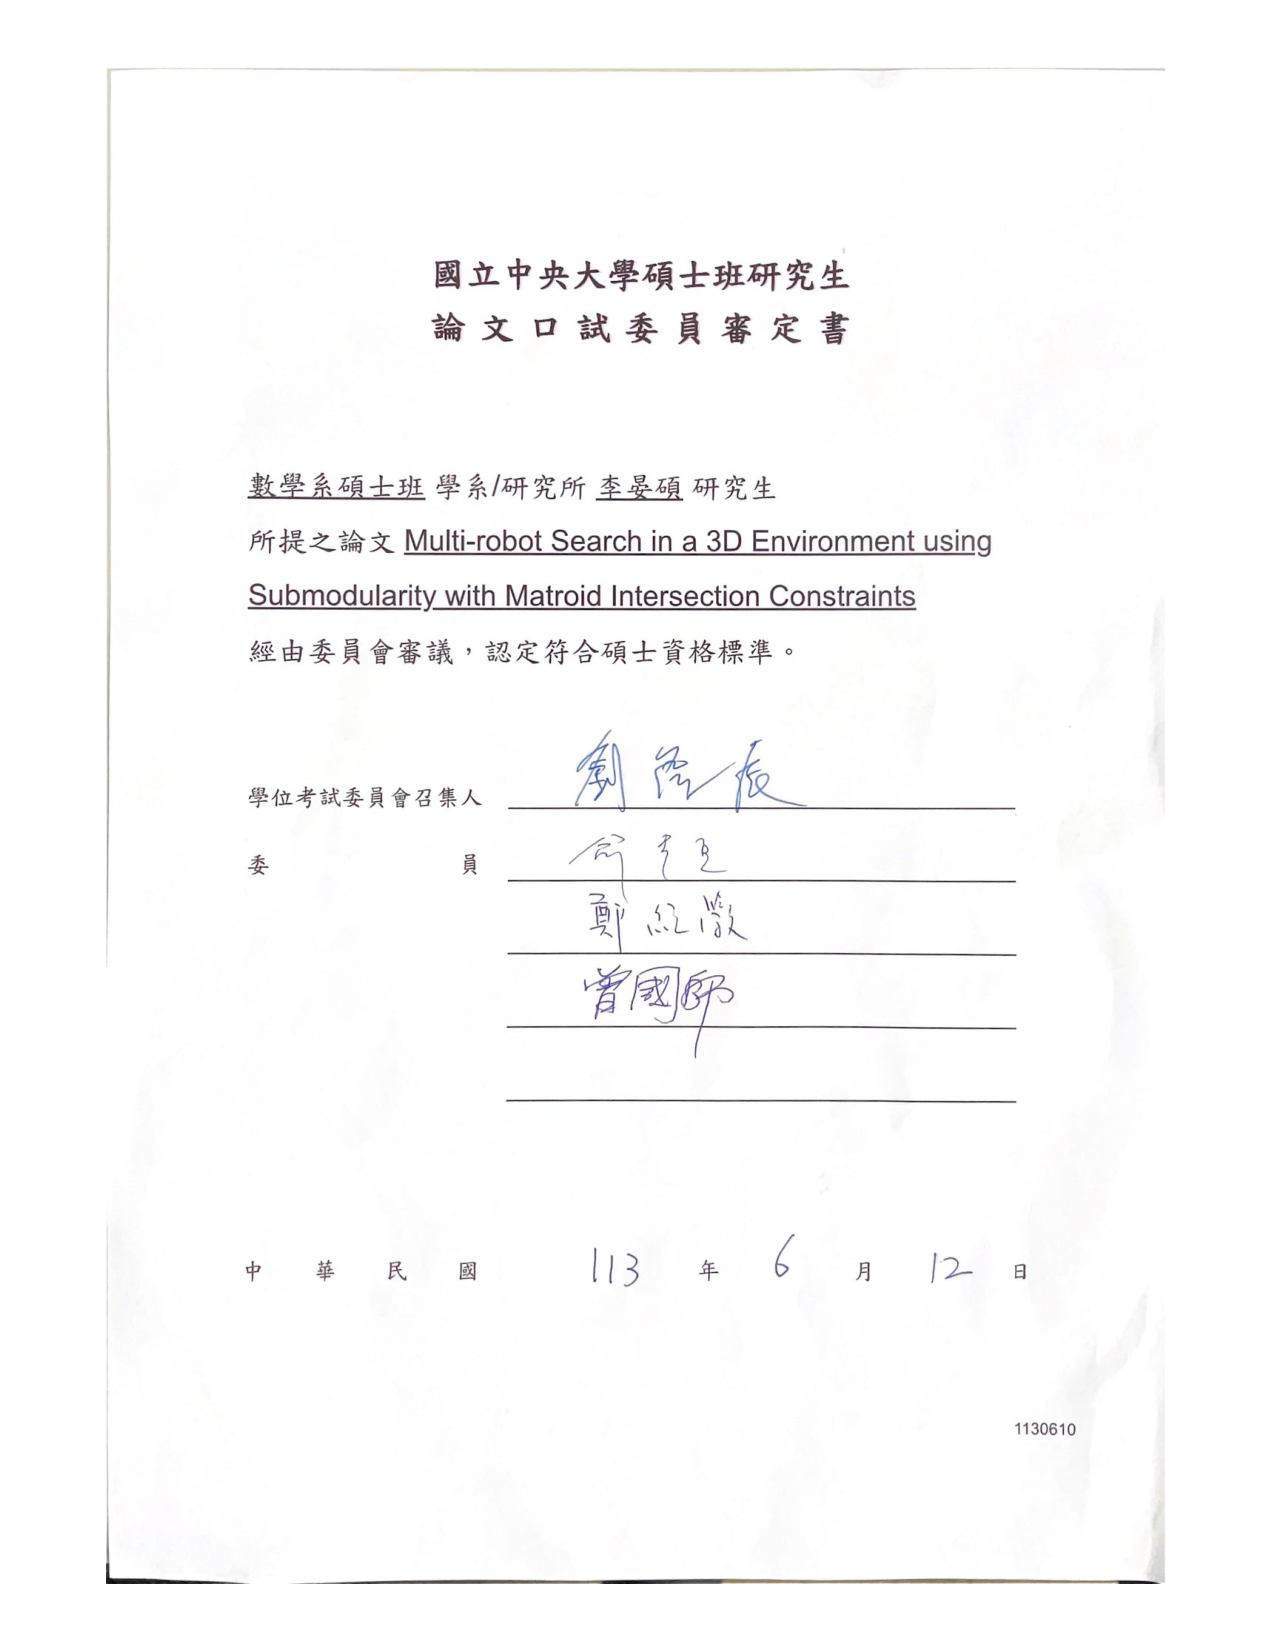
\includepdf[pages=-,scale=0.9]{2.pdf} % 插入其他表格

\pagenumbering{roman}          % 羅馬數字編頁
\title{Multi-robot Search in 3D Environments using Submodularity with Matroid Intersection Constraints}
\begin{abstractcn}
%
\index{ncuthesis 環境!abstractcn}

{\bf \sf 關鍵字:} 次模性, 擬陣理論, 多機器人搜尋問題, 任務分配問題

\vspace{2em}

多機器人搜尋是一個具有挑戰性的問題,因為其涉及任務分配和覆蓋問題,而這些問題皆是NP-hard。
它可以重新定義為在擬陣限制下的覆蓋率最大化問題。
覆蓋率最大化問題可透過次模性來解決。
擬陣限制是由路徑限制和分群限制所組成。
此研究提出Multi-robot Search with Matroid constraints (MRSM)的方法,此方法達成$\frac{1}{3}\widetilde{OPT}$,其中 $\widetilde{OPT}$ 是基於生成樹結構下的近似最優性能。
實驗結果顯示,所提出MRSM方法在多機器人搜尋問題中優於其他演算法。
\end{abstractcn} 
\title{Multi-robot Search in 3D Environments using Submodularity with Matroid Intersection Constraints}
\begin{abstracten}
\index{ncuthesis 環境!abstracten}
{\bf \sf Keywords:} Submodularity, Matroid, Multi-robot search problem, Task allocation problem

\vspace{2em}

The multi-robot search problem is challenging since it involves task allocation and coverage problems, which are NP-hard.
This problem is reformulated as the maximal coverage problem subject to the intersection of matroid constraints.
The coverage problem is solved by utilizing its submodularity.
The intersection matroid is composed of a routing constraint and a clustering constraint.
The proposed algorithm, Multi-robot Search with Matroid constraints (MRSM), achieves $\frac{1}{3}\widetilde{OPT}$, where $\widetilde{OPT}$ is an approximately optimal performance under a spanning tree structure.
The experiment results show that the proposed approach outperforms state-of-the-art methods in multi-robot search problems.
\end{abstracten}

                 % 摘要
%\begin{acknowledgements} \index{Acknowledgements}
\index{ncuthesis 環境!acknowledgements}

感謝指導教授、身邊的親朋好友和所有參與以及協助實驗的人員。
過程中,有你們在一旁鼓勵,真幸福!


%\begin{itemize}
%\end{itemize}
\end{acknowledgements}             % 謝誌
\cleardoublepage
\phantomsection\addcontentsline{toc}{chapter}{Contents}
\tableofcontents                 % toc
\cleardoublepage
\phantomsection\addcontentsline{toc}{chapter}{Figures}
%\renewcommand{\numberline}[1]{圖~#1\hspace*{1em}}%圖目錄
\listoffigures                   % lof
\cleardoublepage
%\renewcommand{\numberline}[1]{表~#1\hspace*{1em}}%表目錄
\phantomsection\addcontentsline{toc}{chapter}{Tables}
\listoftables                    % lot
\index{\LaTeX!\textbackslash phantomsection}
\index{\LaTeX!\textbackslash addcontentline}
\index{\LaTeX!\textbackslash hspace}
\include{symbol}                     % 符號說明     symbols 環境
\cleardoublepage

\pagenumbering{arabic}           % 阿拉伯數字編頁
                                 % \mainmatter
\chapter{Introduction}

Multi-robot search is a widely studied topic due to emerging application domains such as target tracking \cite{schlotfeldt2018anytime}, search and rescue \cite{jennings1997cooperative}, and industrial inspection \cite{correll2009multirobot}.
The multi-robot search problem involves coverage, multi-robot task allocation, and routing problems.
Challenges of these problems are as follows.
First, finding the maximal coverage under a budget is computational intractability \cite{khuller1999budgeted}.
Second, the task allocation to multiple robots is another issue \cite{korsah2013comprehensive}.
Third, each robot in multi-robot search problems needs to solve the traveling salesman problem (TSP) \cite{zhang2016submodular}.
Solving these problems is NP-hard.

Recent approaches to solving these problems are as follows.
For the multi-robot search problem,
the researchers propose an efficient path planning algorithm (eMIP) \cite{singh2007efficient}.
The problem is solved by a sequential single robot path planning algorithm.
Furthermore, each robot needs to solve the TSP, which results in poor time complexity.
A theoretical performance guarantee is provided.
However, the search performance deteriorates as the number of robots increases.
The problem is reformulated as submodular maximization subject to intersection system constraints (MRSIS)\cite{li2024mrsis}.
The search problem is solved by generating a set of robot trajectories while considering the balance of task assignments.
However, it requires solving the minimum spanning tree (MST) problem, and the theoretical performance is not provided.

For multi-robot task allocation problems, Markov Decision Processes (MDP) over graphs are adopted.
In \cite{paull2022learning}, the researchers propose a reinforcement learning algorithm based on a graph neural network.
The task assignment problem is solved by selecting the node with the highest probability for each robot.
However, the routing problem and workload balance are not considered.

\begin{figure}[htbp]
\centerline{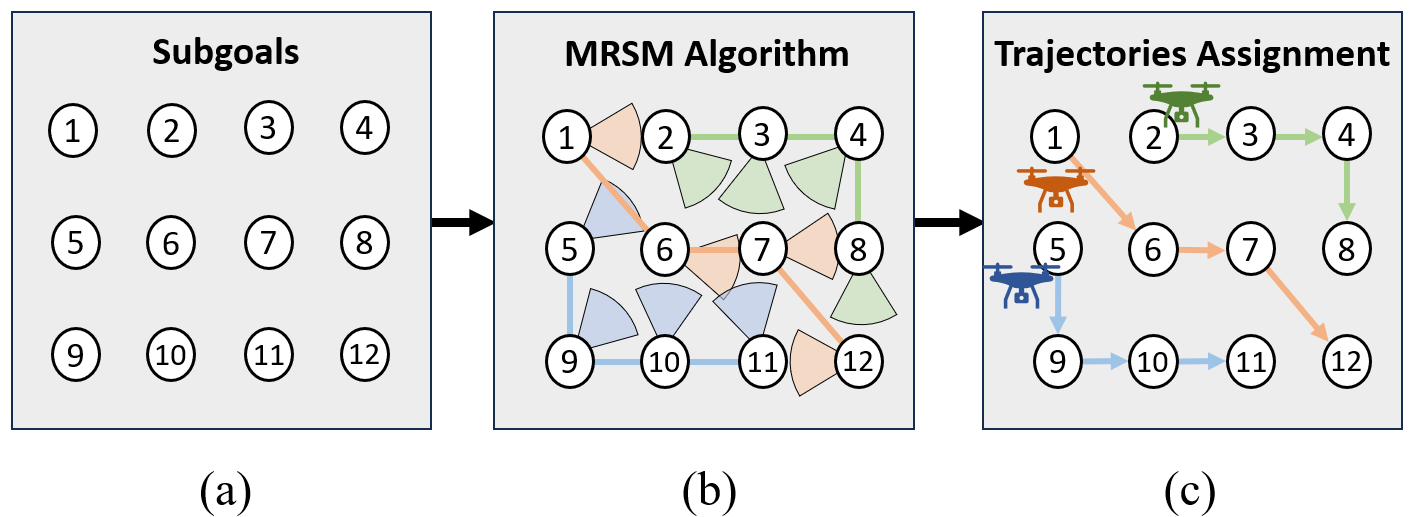
\includegraphics[width=1\textwidth]{overview-2.png}}
\caption{Overview of the proposed multi-robot search system with three robots.
(a) An example of subgoals (nodes) in a search environment.
(b) The trajectories for each robot (orange, blue, and green lines) are obtained by the proposed algorithm (MRSM). The circular sectors are the coverage areas.
(c) The trajectories are assigned to robots to find targets in the environment.
}
\label{overview}
\end{figure}


%\begin{figure}[htbp]
%\centering
%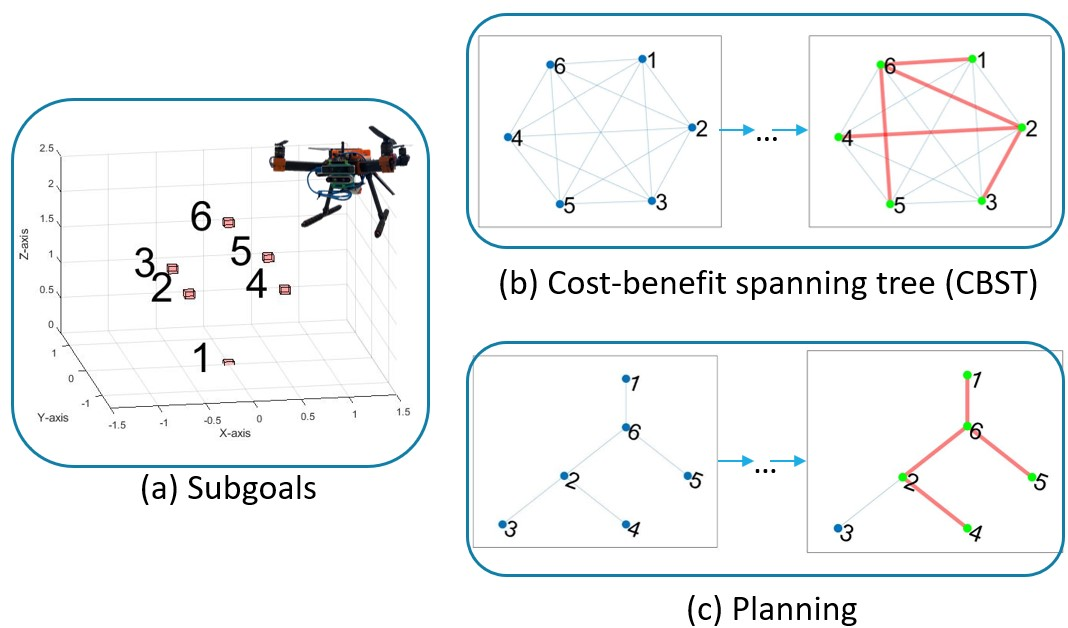
\includegraphics[width=1.0\linewidth]{method_intro.jpg}
%\caption{ Illustration of the proposed method.
%(a) Subgoals.
%The blue points and decimal numbers represent subgoals and the index of subgoals, respectively.
%(b) The cost-benefit spanning tree.
%The green points, red lines and decimal numbers represent nodes in spanning tree, edges in spanning tree and the index of subgoals, respectively.
%(c) Path.
%The green points and red lines represent the path nodes and path edges, respectively.
%}
%%(b) The change of objective function from minimum spanning tree to cost-benefit spanning tree (c) Tree structure of \emph{CBST}.}
%\label{fig:method_intro}
% \end{figure}


For search via learning approaches,
the researchers propose a probability density function (PDF) as a reward function that generates a sequence of decisions based on the reinforcement learning method \cite{sheng2022pd}.
The search problem and the allocation problem are solved by selecting actions with the maximal individual reward function for each robot.
Yet, the graph only considers the unit cost for routing, and the balance of the robots' workloads is not taken into account, potentially resulting in poor task assignment.

To resolve the aforementioned issues, this research proposes a Multi-Robot Search with Matroid constraints (MRSM) algorithm\footnote{The primary distinction between MRSIS and MRSM is that MRSIS models the clustering and routing constraints as independence systems while MRSM models two constraints as matroids.}, which is an improved version of MRSIS algorithm\cite{li2024mrsis}.
Maximal coverage and balanced workloads are considered simultaneously.
The coverage function is to cover a larger area for robots, while the balancing function is to measure the equality of the workloads assigned to robots.
Besides, the routing constraint is reformulated as matroid to boost the theoretical guarantees of the MRSIS \cite{li2024mrsis}.

The proposed MSRM method is illustrated in Fig. \ref{overview}. Given an environment map with subgoals, the goal is to find all targets with multiple robots as soon as possible.
In Fig. \ref{overview}(a), subgoals are evenly distributed in the space. A weighted graph $\mathcal{G}(V,E, w)$ is constructed, where $V$ represents the subgoal set, $E$ represents the edge set, and $w$ is an Euclidean distance function.
In Fig. \ref{overview}(b), the MSRM generates a set of trajectories that maximize the environment coverage and maintain balanced workloads among robots.
In Fig. \ref{overview}(c), trajectories are then assigned to robots to search for targets in the environment.

In this research, some assumptions are made. First, MRSM relies on known environments. A set of subgoals is evenly distributed in the search environments.
Second, the coverage at every subgoal can be pre-computed since the search method is based on known maps.
Third, the perception of robots includes uncertainty and targets may be occluded in the environment.

The contributions of this research are as follows.
First,  the submodular maximization under matroid intersection constraints (MRSM) is proposed for multi-robot search problems.
To the best of our knowledge, this is the first work to propose this objective for these problems.
Second, thanks to the submodularity,
the theoretical guarantees of MRSIS \cite{li2024mrsis} and MRSM are proved as $\frac{1}{2+k_G} \overline{OPT}$ and $\frac{1}{3}\widetilde{OPT}$, respectively, where $k_G > 1$, $\overline{OPT}$ is an approximately optimal solution of the MST or TSP solver and $\widetilde{OPT}$ is an approximately optimal solution of the spanning tree.
Notice that the theoretical bound of MRSM does not depend on the number of robots.
Third, the experiment results show that the proposed method (MRSM) outperforms state-of-the-art approaches (e.g., MRSIS \cite{li2024mrsis}, CapAM \cite{paull2022learning} and PD-FAC \cite{sheng2022pd}) in the multi-robot search problem.

This paper is organized as follows. Section 2 reviews the relevant work on target search methods, multi-robot task allocation, and routing constraints. Section 3 describes the background knowledge of this research. Section 4 introduces the problem formulation. Section 5 describes the search algorithm. Section 6 describes the experiments and analyzes the results. Finally, Section 7 draws conclusions and outlines future work.

\section{Publication Note}
Portions of the literature survey, problem formulation, and experiments appeared in \cite{li2024mrsis}.


               % 第一章
\chapter{Related Work}
In this section, recent work on target search methods, multi-robot task allocation, and routing constraints is reviewed.

\section{Target Search}
Searching for targets in an environment is a sequential decision-making problem. Therefore, search methods based on the type of decision-making algorithm, such as submodular approaches, the frontier-based search, the next-best-view search, the probabilistic search, and Partially Observable Markov Decision Processes (POMDP), can be adopted to generate the search strategies.

The submodular method formulates the target search problem as submodular maximization under a resource constraint.
Singh et al. \cite{singh2007efficient} introduce an efficient path planning algorithm (eMIP), which coordinates multiple robots to obtain highly informative paths subject to the robot's path cost.
The eMIP finds solutions that achieves at least $\frac{1-1/e}{1+\log_2 N}$, where $N$ is the number of robots.
However, the performance deteriorates when more robots are involved.
Li et al. \cite{li2024mrsis} propose a Multi-Robot Search with an Intersection System (MRSIS) algorithm.
The objective is to generate a set of robot trajectories that maximize a coverage function and balance robot workloads under clustering and routing cost constraints.
The clustering and routing constraints are formulated as an intersection system.

The frontier-based search method utilizes the frontier between the explored and unexplored space to expand existing knowledge.
Zhou et al. \cite{zhou2021fuel} propose a hierarchical framework, Fast UAV ExpLoration (FUEL), that supports UAV exploration in complex unknown environments. It improves the exploration efficiency using the incremental frontier information structure.
The work is extended to decentralized multi-UAV\cite{zhou2023racer}.
Instead of allocating frontiers and viewpoints to the UAVs, the task assignment is based on an online hierarchical decomposition to ensure that all UAVs simultaneously explore distinct regions.

The next-best-view (NBV) planning determines the next viewpoint that provides the most valuable information to improve search efficiency.
Mittal et al. \cite{mittal2019vision} adopt NBV planner for exploration and propose a novel landing site detection algorithm that computes costmaps based on several hazard factors (e.g., terrain flatness, steepness, depth accuracy, and energy consumption information).
Lauri et al. \cite{lauri2020multi} propose a submodular utility function for multi-sensor NBV planning under partition matroid constraints. In addition, the utility function coordinates view selection and prevents overlapping views among multiple sensors.

The probabilistic approach is to estimate the target location under sensor and target motion uncertainty.
Robots make decisions based on the probability distribution.
Mohamed et al. \cite{Mohamed2020person} present the person search-orienting problem (PSOP).
It adopts the user activity probability density functions (APDFs) to generate a search plan to maximize the expected target detection with the limited search time. The approach is then extended to multiple robots by generating a team plan to cooperate effectively \cite{Mohamed2022multirobot}.
Sheng et al. \cite{sheng2022pd} propose a probability density factorized (PD-FAC) multi-agent distributional reinforcement learning method that decomposes the PDF of the multi-robot system into a set of individual value distributions. It is guaranteed that the objective function of the overall system’s value distribution can be linearly approximated by the same reliability metric defined over the agent’s individual value distribution.

Formulating robotic search problems as Partially Observable Markov Decision Processes (POMDP) has recently become a popular method.
POMDP considers the search problem where the states of target locations and robot sensors are uncertain.
A sequence of actions is generated by maximizing a reward function.
Zhu et al. \cite{zhu2020approach} propose a Dec-POMDP method to find a target in an environment with obstacles. The approach provides a scalable framework for a large number of UAVs. It enables the UAV swarm to cooperate efficiently by sharing limited observations in the mission.
Many methods constrain the search space in 2D. Zheng et al. \cite{Zheng2021mos3d} present a multi-object search method, 3D Multi-Object Search (3D-MOS), in 3D environments with a frustum-shaped field of view, which can be applied to mobile robots or drones.


\section{Multi-Robot Task Allocation (MRTA)}
The goal of MRTA is to optimize an objective function within a given budget for multiple robots. However, finding an optimal solution is NP-hard \cite{korsah2013comprehensive}.

% matroid
Several research studies have employed submodular maximization with matroid constraints to solve the MRTA problem. This problem involves various challenges, such as the orienteering problem \cite{gunawan2016orienteering}, the intermittent deployment problem \cite{liu2018optimal}, and the capacitated vehicle routing problem \cite{ralphs2003capacitated}.
If the objective function is submodular, greedy algorithms can find solutions with theoretical guarantees\cite{nemhauser1978analysis}.
In the team surviving orienteers (TSO) problem \cite{jorgensen2017matroid},
an independent set of a matroid is selected for maximizing the expected visited nodes at least one robot.
These nodes also ensure that each vehicle reaches its destination with probabilities above a specified threshold.
In environmental monitoring application \cite{liu2019submodular}, the multi-robot task allocation problem and the multi-robot intermittent deployment problem are formulated as submodular maximization with matroid intersection constraints.
In the surveillance task allocation in urban environments \cite{williams2017decentralized}, a decentralized algorithm, which applies auction methods to assign tasks with matroid constraints, is proposed.

% RL
Recent research on multi-robot task allocation has been paying attention to deep reinforcement learning approaches with graph neural network (GNN) \cite{tolstaya2021multi}.
Paul et al. \cite{paull2022learning} propose a Capsule Attention-based Mechanism (CapAM), a graph reinforcement learning architecture that encodes graph information such as robot location, task deadline, and elapsed mission time. The approach can be easily scaled to a large number of tasks.
Tolstaya et al. \cite{tolstaya2021multi} develop a GNN architecture with behavior cloning to solve the coverage problem. Using a sparse representation of the local graph connectivity, the approach can scale to larger maps and teams.
Zhang et al. \cite{zhang2022h2gnn} propose a Hierarchical-Hops Graph Neural Networks (H2GNN), which evaluates the importance of graph nodes at different hops through the multi-head attention mechanism. To improve exploration efficiency, multi-agent reinforcement learning is applied to learn collaborative strategies.


\section{Routing Constraints}
Submodular optimization has been explored with extensive applications in various domains, such as sensor placement \cite{krause2007near}, viral marketing \cite{golovin2011adaptive}, and robotic search problems \cite{Tsai2019spatial}.
To apply submodular optimization in realistic environments, different constraints (e.g., cardinality \cite{nemhauser1978analysis}, additive budget \cite{khuller1999budgeted}, and routing \cite{zhang2016submodular}) must be considered.

Zhang et al. \cite{zhang2016submodular} propose a generalized cost-benefit (GCB) greedy algorithm
to solve two NP-hard problems: monotone submodular maximization and routing path minimization (TSP).
GCB finds solutions that achieves $\frac{1}{2}(1-\frac{1}{e})\widetilde{OPT}$ optimum, where $\widetilde{OPT}$ is the approximated optimum.
However, there is a gap between $\widetilde{OPT}$ and the optimal solution ($OPT$). To improve the theoretical guarantee of GCB, Lin et al. \cite{Lin2023ST} propose Tree-Structured Fourier Supports Set (TS-FSS) algorithms that combine the characteristics of submodularity and sparsity of routing trees to boost the theoretical bound.

Besides, Zhang et al. \cite{zhang2022nonmonontone} investigate the non-monotone submodular maximization with the $k$-independence system routing constraint, where $k$ is loosely upper-bounded by the size of the ground set.
An iterated two-stage algorithm is presented to obatin a $[\frac{1}{4k}, 1+\theta]$-bicriterion approximation solution, where $\theta$ is an error parameter within $(0,1)$.



               % 第二章
\chapter{Background Knowledge}
To formulate a multi-robot search problem, some preliminaries are introduced.
Submodularity (Def. \ref{def:defsubmodular}) and independence system (Def. \ref{def:independence-system}) are adopted to formulate the objective function and the robot constraints, respectively.
The objective function consists of the coverage and balancing function (Thm. \ref{thm:proposed-obj}).
The constraint includes clustering of the search environment (Thm. \ref{thm:clustering-matroid}).
The advantage of formulating the submodular maximization subject to the intersection of an independence system (Thm. \ref{thm:intersection-k-systems}) is that the theoretical guarantee is given (Thm. \ref{thm:intersection-matroid-bound}).
To further improve the performance, Def. \ref{def:matroid} introduces the concept of matroid.\\


\section{Submodularity}

The definition and illustration of submodularity are as follows:

\begin{definition} \label{def:defsubmodular} (Submodularity) \cite{nemhauser1978analysis}
A function $f:2^N \rightarrow \mathbb{R}^+$ is submodular if and only if $\forall S \subseteq T \subseteq N, \forall e \in N \setminus T, \ f(S\cup \{e\}) - f(S) \geq f(T\cup \{e\}) - f(S)$. \\
\end{definition}

Let $S=\{1,2,3\}$ be the ground set and $S_A=\{1\}$, $S_B=\{1,2\}$ be two different sets selected from the ground set, i.e., $S_A \subseteq S_B \subseteq S$. In Fig. \ref{submodularity} (a)(b), if the submodular function $f$ is defined as the coverage function, $f(S_A)$ and $f(S_B)$ depict the regions observed by the camera FOV at locations of $\{1\}$ and $\{1,2\}$.
When a new set $s=\{2\}$ is added to both $S_A$ and $S_B$, the marginal gain of the coverage function $f$ is the additional regions covered, which is the red dashed line area shown in Fig. \ref{submodularity}(c). The diminishing return property suggests that incorporating a set into the smaller set results in a greater marginal gain.\\

%\begin{figure}[htbp]
% \begin{center}
%\begin{subfigure}{.22\textwidth}
%  \centering
%  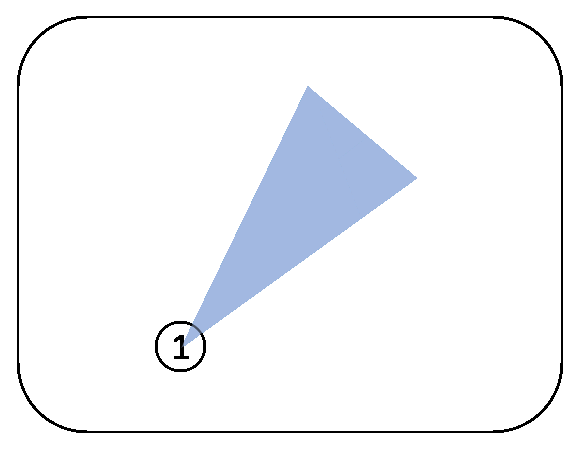
\includegraphics[width=1.0\linewidth]{sub6.eps}
%  \caption{$F(S_A)$}
%\end{subfigure}
%\begin{subfigure}{.22\textwidth}
%  \centering
%  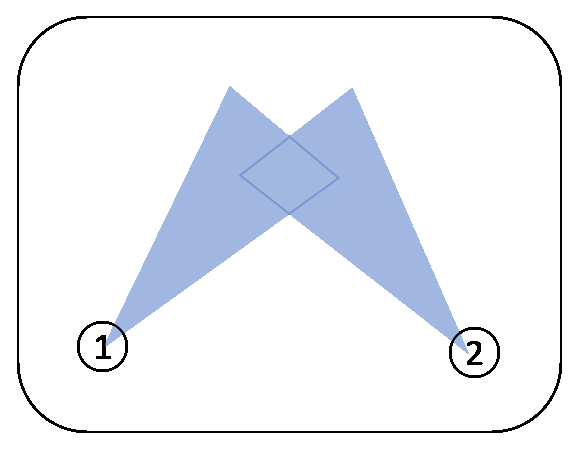
\includegraphics[width=1.0\linewidth]{sub7.eps}
%  \caption{$F(S_B)$}
%\end{subfigure}
%\begin{subfigure}{.44\textwidth}
%  \centering
%  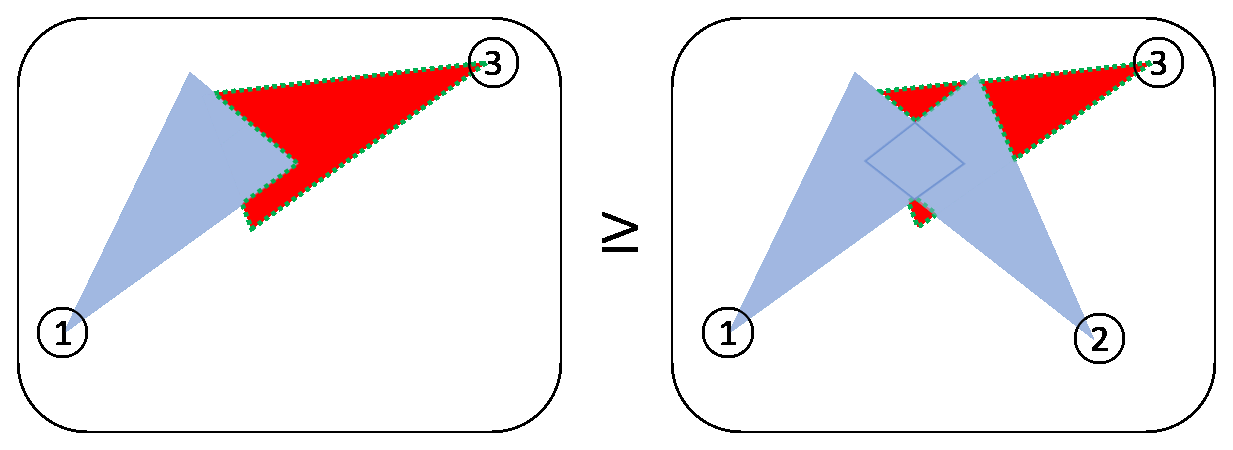
\includegraphics[width=1.0\linewidth]{sub5.eps}
%  \caption{$F(S_A \cup s)-F(S_A)$ and $F(S_B \cup s)-F(S_B)$}
%\end{subfigure}
%\caption{Illustration of submodularity. The decimal number represents the selected sensor.
%The colorful and white areas represent the covered and uncovered areas, respectively.
%(a) $F(S_A)$ represents the covered area by $S_A,$ where $S_A = \{1\}.$ (b) $F(S_B)$ represents the covered area by $S_B,$ where $S_B = \{1, 2\}.$
%(c) The green dash lines represent the submodular gain after adding $s,$ where $s = \{3\}.$ Left figure shows the $F(S_A\cup s) - F(S_A)$ and right figure shows that $F(S_B\cup s) - F(S_B).$}
%\label{fig:submodularity}
% \end{center}
% \end{figure}

\section{Matroid}

\begin{figure}
   \centering
   \begin{subfigure}[b]{0.3\textwidth}
       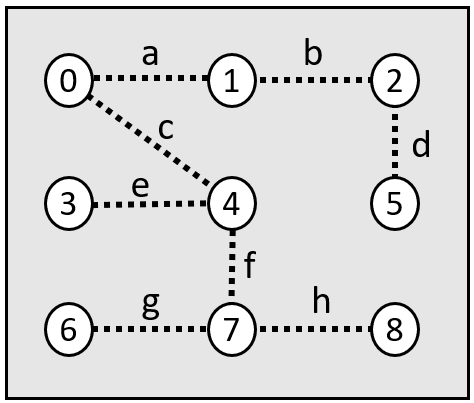
\includegraphics[width=1\textwidth]{def-mat-0.png}
       \caption{Ground set $E$}
   \end{subfigure}
   \hfill
   \quad
   \centering
   \begin{subfigure}[b]{0.3\textwidth}
       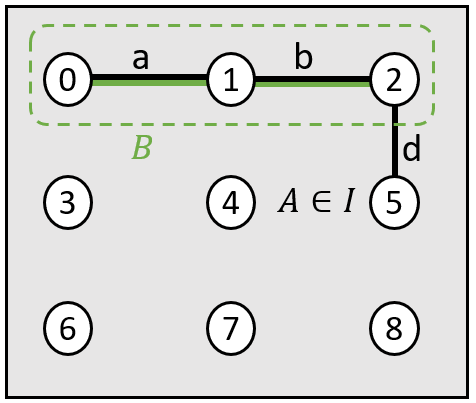
\includegraphics[width=1\textwidth]{def-mat-1.png}
       \caption{$A \in \mathcal{I}$ and $B \subseteq A$}
   \end{subfigure}
   \hfill
   \quad
   \begin{subfigure}[b]{0.3\textwidth}
   \centering
       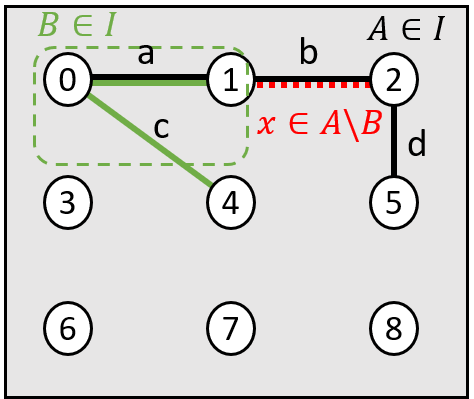
\includegraphics[width=1\textwidth]{def-mat-2.png}
       \caption{$|A|>|B|$}
   \end{subfigure}
   \hfill

   \caption{Illustration of the downward closure and the exchange property.
   The vertices represent the geographic locations of sensors, and the edges are the distance between two vertices. (a) The ground set $E=\{a,b,c,d,e,f,g,h\}$ (the black dashed lines) (b) $A=\{a,b,d\}$ (the black solid lines) is a set that satisfies the independent set $\mathcal{I}$. $B=\{a,b\}$ (the green solid lines) is a subset of $A$.
   (c) Two sets $A=\{a,b,d\}$ (the black solid lines) and $B=\{a,c\}$ (the green solid lines) satisfy the independent set $\mathcal{I}$, where $|A|>|B|$. Then there exists an element $x \in A \setminus B$ such that adding to the smaller set $B$ still satisfies the condition of the independent set $\mathcal{I}$, e.g., $x=b$ (the red dashed lines).
   }
   \label{def-matroid}
\end{figure}

\begin{definition} \label{def:independence-system} (Independence System) \cite{korte1978analysis}
An independence system is a pair $(E, \mathcal{I})$, where $E$ is a finite set called the ground set and $\mathcal{I}$ is a family of subsets of $E$ called independent sets such that:
\begin{enumerate}
    \item (non-emptiness) $\emptyset \in \mathcal{I}$;
    \item (downward closure) if $A\in \mathcal{I}$ and $B \subseteq A$, then $B \in \mathcal{I}$. \\
\end{enumerate}

An illustrative example is as follows.
Consider a ground set $E=\{a,b,c,d,e,f,g,h\}$ and an independent set $\mathcal{I}=\{\{a,b,c\}, \{a,b,d\}, \{a,b\}, \\ \{a,c\}, \{a,d\}, \{b,c\}, \{b,d\}, \{a\}, \{b\}, \{c\}, \{d\}, \emptyset \}$, shown in Fig. \ref{def-matroid}(a).
Let $A \in \mathcal{I}$ be a set, and $B \subseteq A$ be a subset. In Fig. \ref{def-matroid}(b), the downward closure property states that if $A\in \mathcal{I}$ and $B \subseteq A$, then $B \in \mathcal{I}$.\\
\end{definition}

\begin{definition} \label{def:k-independence-system} ($k$-independence System) \cite{korte1978analysis}
Given a ground set $E$, an independence family $\mathcal{I}$ and a set $Y\subset E$. Let $r(Y)$ be the set of maximal elements of $\mathcal{I}$ which are subsets of $Y$. That is, $r(Y)=\{A \in \mathcal{I} | A\subseteq Y \text{ and there is no }A' \in \mathcal{I} \text{ such that } A\subset A' \subseteq Y \}$. Then $(E, \mathcal{I})$ is a $k$-independence system if for all $Y\subset E$,
\begin{align*}
    \frac{\max_{A\in r(Y)}|A|}{\min_{A\in r(Y)}|A|} \leq k,
\end{align*}
where $k\geq1$. As a special case, if $k=1$, then $(E, \mathcal{I})$ is a matroid. \\
\end{definition}

\begin{definition} \label{def:matroid} (Matroid) \cite{nemhauser1978analysis}
A matroid $\mathcal{M}$ is a pair $(E, \mathcal{I})$, where $E$ is a finite set called the ground set and $\mathcal{I}$ is a family of subsets of $E$ called independent sets, with the following properties:
\begin{enumerate}
    % \item (non-emptiness) $\emptyset \in \mathcal{I}$;
    \item (downward closure) if $A\in \mathcal{I}$ and $B \subseteq A$, then $B \in \mathcal{I}$;
    \item (exchange property) if $A \in \mathcal{I}, B\in \mathcal{I}$ and $|A|>|B|$, then there exists $x \in A\setminus B$ such that $B \cup \{x\} \in \mathcal{I}$.\\
\end{enumerate}
\end{definition}

An example of a matroid $\mathcal{M}=(E, \mathcal{I})$ is illustrated in Fig. \ref{def-matroid}.
Consider a ground set $E=\{a,b,c,d,e,f,g,h\}$ and an independent set $\mathcal{I}=\{\{a,b,c\}, \{a,b,d\}, \{a,b\}, \{a,c\}, \{a,d\}, \{b,c\}, \{b,d\}, \{a\}, \\ \{b\}, \{c\}, \{d\}, \emptyset \}$ in Fig. \ref{def-matroid}(a).
Let $A \in \mathcal{I}$ be a set and $B \subseteq A$ be a subset, shown in Fig. \ref{def-matroid}(b). The downward closure property states that if $A\in \mathcal{I}$ and $B \subseteq A$, then $B \in \mathcal{I}$. In Fig. \ref{def-matroid}(c), consider two sets $A \in \mathcal{I}$ and $B \in \mathcal{I}$, where $|A|>|B|$. By the exchange property, there exists an element $x \in A\setminus B$ such that $B+x \in \mathcal{I}$.\\

\begin{theorem} \label{thm:intersection-k-systems} (Intersection of independence systems) \cite{mestre2015intersection}
The intersection of a $k_1$-independence system and a $k_2$-independence system is a $(k_1 + k_2)$-independence system. \\
\end{theorem}

To illustrate the concept, let $(E, \mathcal{I}_1)$ and $(E, \mathcal{I}_2)$ be a $k_1$-independence system and a $k_2$-independence system, respectively.
The goal is to find the intersection of $(E, \mathcal{I}_1)$ and $(E, \mathcal{I}_2)$, namely $(E, \mathcal{I}_1 \cap \mathcal{I}_2)$. Then $(E, \mathcal{I}_1 \cap \mathcal{I}_2)$ is a $(k_1 + k_2)$-independence system. \\

\begin{theorem} \label{thm:intersection-matroid} (Intersection of matroids) \cite{nemhauser1978analysis}
Consider the matroid intersection system

\begin{align} \label{eq:inter-matroid}
    \bigcap_{\mathcal{M}\in \mathit{\mathbb{M}}} \mathcal{M} \triangleq\left ( \mathcal{V},\ \bigcap_{\mathcal{M}\in \mathit{\mathbb{M}}} \mathcal{M} \right )
\end{align}

where $\mathit{\mathbb{M}}$ is a set of matroidal independence systems, $\mathcal{M}$ is a matroid, and $\mathcal{V}$ is a ground set. Eq. \eqref{eq:inter-matroid} models any arbitrary independence system. \\
\end{theorem}

\begin{theorem} \label{thm:intersection-matroid-bound} (Theoretical bound of a matroid intersection) \cite{fisher1978analysis}
Given a submodular monotone set function $F$ and a set of matroidal independence systems $\mathit{\mathbb{M}}$, maximizing $F$ under an intersection of matroids with the greedy algorithm yields a solution $X$. The performance of the set $X$ is

\begin{align*} \label{eq:inter-matroid}
    F(X) \geq \frac{1}{|\mathit{\mathbb{M}}|+1} F(X^{opt}),
\end{align*}
where $|\mathit{\mathbb{M}}|$ is the cardinality of $\mathcal{M}$ and $X^{opt}$ is an optimal solution. \\
\end{theorem}

Consider a set of matroidal independence systems $\mathit{\mathbb{M}} = \{\mathcal{M}_1, \mathcal{M}_2\}$.
The cardinality of $\mathit{\mathbb{M}}$ is $2$.
Therefore, greedy algorithms find a solution $X$ such that the performance of $X$ achieves $\frac{1}{3} F(X^{opt})$.\\

In multi-robot search scenarios, the search environment must be partitioned into smaller segments to accommodate multiple robots.
Ensuring an equitable distribution of workloads among robots is a key consideration for efficient task assignments.
Therefore, the coverage and balancing function \cite{li2024mrsis} and the clustering constraint \cite{liu2013entropy} are introduced. \\

\begin{theorem} \label{thm:clustering-matroid} (Clustering constraint) \cite{liu2013entropy}
Let $E$ be the edge set and $S \in E$ be the set of subsets. $\mathcal{M}_C=(E, \mathcal{I}_C)$ is matroidal, where $\mathcal{I}_C=\{S \subseteq E : N \geq n \}$, $N$ is the number of clusters, and $n$ is the clustering budget. \\
\end{theorem}

\begin{theorem} \label{thm:proposed-obj} (Submodularity of a coverage and balancing function) \cite{li2024mrsis}
Let $S$ be a set, $\lambda \in [0,1]$ be a constant, $f:2^S \rightarrow \mathbb{R}^+$ be a coverage function, and $\mathcal{B}: 2^S \rightarrow \mathbb{R}^+$ be a balancing function.
The coverage and balancing function $F(S)=f(S)+\lambda \mathcal{B}(S)$ is submodular. \\
\end{theorem}

\begin{theorem} \label{thm:balance} (Submodularity of balancing function) \cite{liu2013entropy}
 Given a graph $\mathcal{G}=(V, E)$ and a partition set $S=\{S_i \in V : i\in \{1,...,N\}\}$, the balancing function $\mathcal{B}:2^E \rightarrow \mathbb{R}$ is a monotonically increasing submodular function and is defined as follows:
 \begin{align*}
     \mathcal{B}(S)=-\sum_{i} {p_S(i)\log({p_S(i)})-N},
 \end{align*}
 where $p_S(i)=\frac{|S_i|}{|V|}, i=\{1,...,N\}$ and $N$ is the number of connected components in the graph.

 The balancing function encourages the clusters to have similar sizes. Fig. \ref{balancing-func} shows the balancing function of two topologies. The balancing function shown in Fig. \ref{balancing-func}(a) has a higher value compared to that in Fig. \ref{balancing-func}(b). In other words, the higher balancing value has more balanced clustering.\\
\end{theorem}

\begin{figure}
    \centering
    \begin{subfigure}[b]{0.4\textwidth}
    \centering
        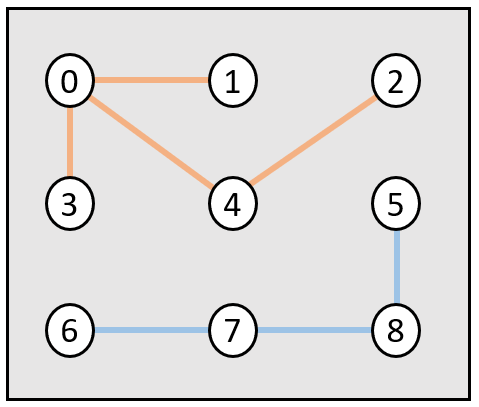
\includegraphics[width=1\textwidth]{-1.01.png}
        \caption{$\mathcal{B}(S_A)=-1.01$}
    \end{subfigure}
    \hfill
    \quad
    \begin{subfigure}[b]{0.4\textwidth}
        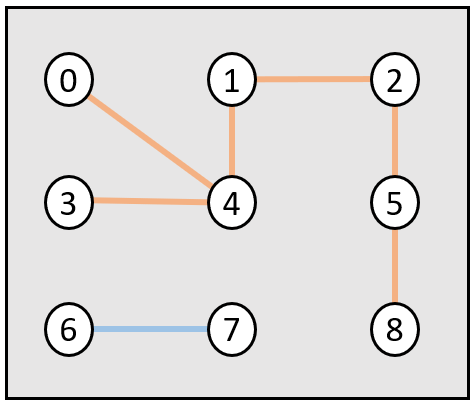
\includegraphics[width=1\textwidth]{-1.24.png}
        \caption{$\mathcal{B}(S_B)=-1.24$}
    \end{subfigure}
    \hfill

    \caption{Illustration of the balancing function. Two clusters are denoted by orange and blue colors. (a) $\mathcal{B}(S_A)$ is the balancing value of $S_A$, where $S_A=\{S_1,S_2\}$, $S_1=\{0,1,2,3,4\}$ and $S_2=\{5,6,7,8\}$. (b) $\mathcal{B}(S_B)$ is the balancing value of $S_B$, where $S_B=\{S_1,S_2\}$, $S_1=\{0,1,2,3,4,5,8\}$, and $S_2=\{6,7\}$.
    }
    \label{balancing-func}
\end{figure}

               % 第三章
\chapter{Problem Formulation}
Given a weighted graph $\mathcal{G}=(V, E, w)$ and an objective function $F:2^E \rightarrow \mathbb{R}^+$, where $V$ is a set of vertex, $E$ is a set of edges and $w:E \rightarrow \mathbb{R}^+$ is a distance function, the goal is to find a subset $S \subseteq E$ that maximizes environmental coverage and balances robot workloads subject to a constraint.
The objective function $F(S)=f(S)+\lambda \mathcal{B}(S)$ \cite{li2024mrsis} is defined as a linear combination of a coverage function $f$ and a balancing function $\mathcal{B}$, where $\lambda \in [0,1]$ is the weight of the balancing function\footnote{Both $f$ and $\mathcal{B}$ functions are normalized.}.
In 3D environments, the coverage function is defined by calculating the ratio of the number of covered voxels to the total number of environmental voxels.

Two variant formulations with known world maps are considered: Multi-robot search with independence system (MRSIS) \cite{li2024mrsis} and Multi-robot search with matroid (MRSM). \\

\section{Multi-robot search with independence system (MRSIS)}
\begin{problem} \label{prob:objective-IS}
    (MRSIS) \cite{li2024mrsis} Given an objective function $F$, a set of independence system $\mathit{\mathbb{I}} = \{I_G , I_C\}$, the number of robots $n \in \mathbb{N}^+$, and a set of routing constraints for each robot $l = \{l_i \in \mathbb{R}^+\}_{i=1}^n$, find a subset $S \subseteq E$ that maximizes $F$ under an intersection of independence systems
    \begin{equation} \label{eq:objective-IS}
        \begin{aligned}
            \max_{S} \quad & F(S) \\
            \textrm{s.t.} \quad & S \in \bigcap_{I \in \mathit{\mathbb{I}}} I,
        \end{aligned}
\end{equation}
\end{problem}

The intersection system $\bigcap_{I \in \mathit{\mathbb{I}}} I$ is defined as an intersection of all elements in the set of independence systems.
$\mathit{\mathbb{I}} = \{I_G , I_C\}$ is defined as a set of independence systems, where $I_G=(E, \mathcal{I}_G)$ models the robots' routing constraint and $I_C=(E, \mathcal{I}_C)$ models the cluster constraint.\\


The following theorems and corollaries prove that the routing and clustering constraints are $k$-independence systems.
Then, the theoretical performance guarantee of MRSIS \cite{li2024mrsis} is provided.


\begin{theorem} \label{thm:general-routing} (Routing constraint of a $k$-independence system)
The routing constraint for multiple robots $I_G=(E, \mathcal{I}_G)$ is a $k_G$-independence system, where $k_G > 1$. The independent set is defined as $\mathcal{I}_G=\{S \subseteq E : c(S \cap X_i) \leq l_i , \forall i\in \{1,...,n\}\}$, where $c:2^E \rightarrow \mathbb{R}^+$ is a routing cost function (e.g., TSP or MST solver), $X_i \subseteq S$ is the set of $i^{th}$ cluster and $l_i$ is a routing budget.
\end{theorem}
\begin{proof}
To prove that $I_G$ is an independence system, two properties described in Def. \ref{def:independence-system} must hold.

\textbf{(Non-emptiness property)} Consider a set $B_1=\emptyset$.
Let $A=\{1,...,n\}$ and $m_i=c(B_1 \cap X_i), \forall i\in A$ be the routing costs of the $i$-th cluster and $X_i$ be a set of cluster $i$. Since $B_1$ is an empty set, it implies that $m_i=0, \forall i\in A$. Thus, $B_1$ belongs to the independent set $\mathcal{I}_G$.

\textbf{(Downward closure property)} Consider a set $B_1\subseteq E$ and $B_1 \in \mathcal{I}_G$. Let $m_i=c(B_1 \cap X_i), \forall i\in A$ be the routing costs of the $i$-th cluster and $X_i$ be a set of cluster $i$.
Since $B_1 \in \mathcal{I}_G$, this implies that $c(B_1 \cap X_i) \leq l_i, \forall i\in A$. Therefore, $m_i \leq l_i, \forall i\in A$. Let $B_2 \subseteq B_1$ and $n_i=c(B_2 \cap X_i), \forall i\in A$. Since $B_2$ contains edges no more than $B_1$, the routing costs $n_i \leq m_i$. As a result, $n_i \leq m_i \leq l_i$. Therefore, $B_2$ belongs to the independent set $\mathcal{I}_G$.

Since the independent set $\mathcal{I}_G$ satisfies the non-emptiness and downward closure properties, $I_G=(E, \mathcal{I}_G)$ is a $k_G$-independence system. If $I_G$ does not satisfy the exchange property (Def. \ref{def-matroid}), $k_G$ will be greater than 1.

To prove that $k_G > 1$, consider two sets $B_1\in \mathcal{I}$ and $B_2 \in \mathcal{I}$, where $|B_1|>|B_2|$.
Let $s=B_1 \setminus B_2$, $m_i=c(B_1 \cap X_i)\leq l_i, \forall i\in A$ and $n_i=c(B_2 \cap X_i)=l_i, \forall i\in A$. If $X \notin \emptyset$, adding any element $x \in X$ to $B_2$ forms a new set $B_2'$. It is obvious that $B_2' \notin \mathcal{I}$ since $n_i=l_i \leq c(B_2' \cap X_i)$.
Therefore, $I_G$ does not satisfy the exchange property. $k_G$ is greater than 1.
\\
\end{proof}

\begin{corollary} \label{cor:clustering-indep-sys} (Clustering constraint as a $1$-independence system)
Let $E$ be an edge set and $S \subseteq E$ be a subset.
$I_C=(E, \mathcal{I}_C)$ is an $1$-independence system, where $\mathcal{I}_C=\{S \subseteq E : N \geq n \}$, $N$ is the number of clusters, and $n$ is the number of robots.
\end{corollary}
\begin{proof}
Since $I_C$ is a matroid (Thm. \ref{thm:clustering-matroid}) and matroid satisfies the properties of the independence system (Def. \ref{def:independence-system}),
the clustering constraint $I_C$ is an $1$-independence system.
\\
\end{proof}

\begin{theorem}  \label{def:independence-bound}
 (Lower bound of MRSIS\cite{li2024mrsis}) Let $F$ be the coverage and balancing function, $\mathit{\mathbb{I}}$ be a set of $k$-independence systems, $S$ be the solution of maximizing $F$ subject to the intersection of $\mathit{\mathbb{I}}$ via greedy algorithms. The performance of $S$ is
\begin{equation*}
      F(X) \geq \frac{1}{2+k_G} F(\overline{X^{opt}}),
\end{equation*}
where $k_G > 1$ and $\overline{X^{opt}}$ is an approximately optimal solution depending on the TSP or MST solver.
\end{theorem}
\begin{proof}
In Thm. \ref{thm:proposed-obj}, the coverage and balancing function $F$ satisfies the submodularity.
Let $\mathit{\mathbb{I}}=\{I_C, I_G\}$ be a set of $k$-independence systems. In Cor. \ref{cor:clustering-indep-sys}, the clustering constraint $I_C$ is a $1$-independence system. In Thm. \ref{thm:general-routing}, the general multi-robot routing constraint $I_G$ is a $k_G$-independence system.
By Thm. \ref{thm:intersection-k-systems}, the performance of MRSIS \cite{li2024mrsis} achieves $\frac{1}{2+k_G}\overline{OPT}$, where $\overline{OPT}$ is an approximately optimal solution that depends on the routing cost function.
\\
\end{proof}

To improve the performance of MRSIS \cite{li2024mrsis}, the set of independence systems is reformulated into the set of matroids.

\section{Multi-robot search with matroid (MRSM)}

\begin{problem} \label{prob:objective-Mat}
    (MRSM) Given an objective function $F$, a set of matroidal independence systems $\mathit{\mathbb{M}} = \{\mathcal{M}_R , \mathcal{M}_C\}$, the number of robots $n \in \mathbb{N}^+$, and a set of routing constraints for each robot $l = \{l_i \in \mathbb{R}^+\}_{i=1}^n$, find a set $S \subseteq E$ that maximizes $F$ under an intersection of matroidal independence systems
    \begin{equation} \label{eq:objective-Mat}
        \begin{aligned}
            \max_{S} \quad & F(S) \\
            \textrm{s.t.} \quad & S \in \bigcap_{\mathcal{M}\in \mathit{\mathbb{M}}} \mathcal{M},
        \end{aligned}
\end{equation}
\end{problem}

$\mathit{\mathbb{M}} = \{\mathcal{M}_R , \mathcal{M}_C\}$ is defined as a set of matroidal independence systems, where $\mathcal{M}_R=(E, \mathcal{I}_R)$ and $\mathcal{M}_C=(E, \mathcal{I}_C)$ are the robots routing constraint under tree structure and the clustering constraint, respectively.

The routing matroid $\mathcal{M}_R$ constrains the trajectory length of robots while constructing spanning trees.
The independent set $\mathcal{I}_R$ is a subset of $E$ which satisfies:
\begin{enumerate}
    \item $T \subset S$, where $T \subseteq E$ and $S \subseteq E$ are acyclic, and $|T| < |S|$,
    \item $c_{st}(S \cap X_i) \leq l_i , \forall i\in \{1,2,...,n\}$.
\end{enumerate}
where $X_i \subseteq S$ is the set of the $i^{th}$ cluster and $c_{st}:2^E \rightarrow \mathbb{R}^+$ is a routing cost function for a spanning tree.

The clustering matroid $\mathcal{M}_C$ is defined the same as in MRSIS \cite{li2024mrsis}.
The independent set $\mathcal{I}_C$ is defined as
\begin{align*}
    \mathcal{I}_C=\{S \subseteq E : N \geq n \},
\end{align*}
where $N$ is the number of clusters and $n$ is the number of robots. \\

The following Theorems introduce matroid constraints and the theoretical performance guarantee of MRSM.

\begin{theorem} \label{thm:routing-matroid} (Routing constraint under tree structure)
Let $E$ be an edge set and $T$ and $S$ be any subset of $E$. $\mathcal{I}_R$ is the set of subsets, $S\subseteq E$, which satisfies:
\begin{enumerate}
    \item $T \subset S$, where $T$ and $S$ are acyclic and $|T| < |S|$,
    \item $c_{st}(S \cap X_i) \leq l_i , \forall i\in \{1,...,n\}$, where $c_{st}:2^E \rightarrow \mathbb{R}^+$ is a routing cost function for a spanning tree, $X_i \subseteq S$ is the set of $i^{th}$ cluster and $l_i$ is a routing budget.
\end{enumerate}

The routing constraint $\mathcal{M}_R=(E, \mathcal{I}_R)$ is a matroid.
\end{theorem}
\begin{proof}
To prove that $\mathcal{M}_R$ is a matroid, two properties described in Def. \ref{def:matroid} must hold.

\textbf{(Downward closure property)} Consider a set $B_1\subseteq E$ and $B_1 \in \mathcal{I}_R$.
Let $A=\{1,...,n\}$ and $m_i=c_{st}(B_1 \cap X_i), \forall i\in A$ be the routing costs of the $i$-th cluster, and $X_i$ be the set of the $i$-th cluster.
Since $B_1 \in \mathcal{I}_R$, this implies that $B_1$ is a tree (acyclic graph) and $m_i \leq l_i, \forall i\in A$.
Let $B_2 \subseteq B_1$ and $n_i=c_{st}(B_2 \cap X_i), \forall i\in A$.
Since $B_2$ contains edges no more than $B_1$, the routing costs must be $n_i \leq m_i$.
In addition, removing any edge from $B_1$ forms $B_2$ which does not form a cycle.
As a result, $n_i \leq m_i \leq l_i$ and $B_2$ is acyclic.
Therefore, $\mathcal{I}_R$ satisfies the downward closure property.

\textbf{(Exchange property)} Consider two sets $B_1 \in \mathcal{I}_R$ and $B_2\in \mathcal{I}_R$, where $|B_1|>|B_2|$.
Since $B_1$ and $B_2$ satisfy the condition of the independent set and $|B_1|>|B_2|$, it implies that $B_2 \subset B_1$.
Let $m_i=c_{st}(B_1 \cap X_i)$ and $n_i=c_{st}(B_2 \cap X_i), \forall i\in A$.
If $B_2 \subset B_1$, it is clear that $n_i \leq m_i \leq l_i$.
Besides, removing any edge from $B_1$ forms $B_2$, which is acyclic.
Therefore, $\mathcal{I}_R$ satisfies the exchange property.

Since the independent set $\mathcal{I}_R$ satisfies the downward closure properties and the exchange property, $\mathcal{M}_R=(E, \mathcal{I}_R)$ is a matroid.\\
\end{proof}

\begin{definition}
    (Matroidal independence systems of routing and clustering constraints) Given a tree-structured routing constraint $\mathcal{M}_R$ with a set of routing budgets $\{l_i\}_{i=1}^n$ and a clustering constraint $\mathcal{M}_C$ with $n$ robots. A set of matroidal independence systems is defined as $\mathit{\mathbb{M}} = \{\mathcal{M}_R , \mathcal{M}_C\}$.\\
\end{definition}

The routing matroid $\mathcal{M}_R$ constrains the trajectory length of robots via constructing spanning trees while the clustering matroid $\mathcal{M}_C$ divides the ground set into groups for robots.

To illustrate the concept, two cases are illustrated as follows.
Fig. \ref{independent-set} illustrates the intersection system of $\mathcal{M}_R=(E, \mathcal{I}_R)$ and $\mathcal{M}_C=(E, \mathcal{I}_C)$.
Let $E$ be the set of edges between any vertex, $(a,b)\in E$ be an undirected edge, $\mathit{\mathbb{M}}=\{\mathcal{M}_R, \mathcal{M}_C\}$ be the set of matroidal independence systems, $l_i=10$ be the routing constraint and $n=3$ be the minimum number of clusters. In Fig. \ref{independent-set}(a), let $S_A=\{S_1,S_2,S_3\}$, where $S_1=\{(0,4)\},S_2=\{(3,5)\},$ and $S_3=\{(6,7),$$(7,8)\}$. $S_A$ satisfies the intersection system since $S_A$ is acyclic, $|S_A|\geq n$ and $c(S_A \cap S_i) \leq l_i$, where $i=\{1,2,3\}$.
In Fig. \ref{independent-set}(b), let $S_B=\{S_1,S_2\}$, where $S_1=\{(0,4),(4,2),(2,5),(3,5)\}$ and $S_2=\{(6,7),$$(7,8)\}$. $S_B$ does not satisfy the intersection system since $|S_B| < n$ and $c(S_B \cap S_1) > l_i$. \\

\begin{figure}
    \centering
    \begin{subfigure}[b]{0.4\textwidth}
        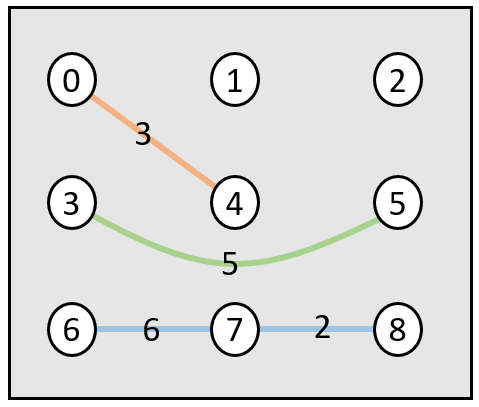
\includegraphics[width=1\textwidth]{mat-1.png}
        \caption{$S_A \in \bigcap_{\mathcal{M}\in \mathit{\mathbb{M}}} \mathcal{M}$}
    \end{subfigure}
    \hfill
    \quad
    \begin{subfigure}[b]{0.4\textwidth}
    \centering
        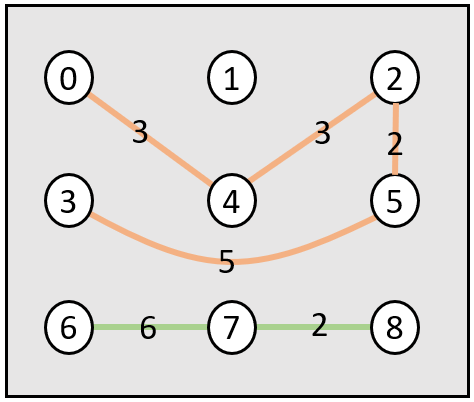
\includegraphics[width=1\textwidth]{mat-2.png}
        \caption{$S_B \not \in \bigcap_{\mathcal{M}\in \mathit{\mathbb{M}}} \mathcal{M}$}
    \end{subfigure}

    \caption{Illustration of the intersection system.
    The vertices and lines represent the subgoals and the distances between two vertices, respectively.
    Each color line denotes a cluster. (a) $S_A$ contains three clusters that satisfy the condition of the intersection system. (b) $S_B$ contains two clusters that violate the condition of the intersection system due to the under-budget of the clustering and the over-budget of routing constraints.
    }
    \label{independent-set}
\end{figure}

\begin{theorem}  \label{def:proposed-bound}
 (Lower bound of the proposed algorithm for MRSM) Let $F$ be the coverage and balancing function, $\mathit{\mathbb{M}}$ be a set of matroidal independence systems, $S$ be the solution of maximizing $F$ subject to the intersection of $\mathit{\mathbb{M}}$ via greedy algorithms. The performance of $S$ is
\begin{equation*}
      F(X) \geq \frac{1}{3} F(\widetilde{X^{opt}}),
\end{equation*}
where $\widetilde{X^{opt}}$ is the optimal solution under tree structure.
\end{theorem}
\begin{proof}
The coverage and balancing function $F$ is submodular (Thm. \ref{thm:proposed-obj}) and each element in $\mathit{\mathbb{M}}$ is a matroid (Thm. \ref{thm:clustering-matroid} and Thm. \ref{thm:routing-matroid}).
By Thm. \ref{thm:intersection-matroid-bound}, the performance of the proposed method is guaranteed to find a solution that achieves $\frac{1}{3}\widetilde{OPT}$, where $\widetilde{OPT}$ is the optimal performance under tree structure.
\end{proof}

               % 第四章
\chapter{Proposed algorithms}
There are two algorithms: CBST algorithm and terrain monitoring algorithm.
The Alg.~\ref{al:CBST} is to generate the CBST (e.g., from Fig.~\ref{fig:method_intro} (a) to Fig.~\ref{fig:method_intro} (b)).
The Alg.~\ref{al:TM_CBST} is to generate the path using GCB algorithm (e.g.,  from Fig.~\ref{fig:method_intro} (b) to Fig.~\ref{fig:method_intro} (c)).


In Alg.~\ref{al:CBST}, the inputs are an undirected graph ($G$), the source ($s$).
The output is the spanning tree.
Line $1$ is to build $Q$ (vertices in $G$).
Lines $2-3$ are initialization{\color{olive}s}.
Line $5$ is to find the distance connecting $v_q$ and $v_k$, where $v_q$ belongs to the current growing tree ($S$), and $v_k$ does not belong to the tree current growing tree.
Line $6$ is to find the path length from the source vertex to $v_q$ along the current growing tree ($S$).
Line $7$ is to maximize $f/c$, where $c$ is the cost function about Prim's algorithm and Dijkstra algorithm.
Lines $8-9$ are to update current tree and spanning tree.


\begin{algorithm}[htbp]	
	\KwIn{\\
$G = (V, E, w)$: undirected graph \\
$s$: the start point \\
$f$: objective function
}
\KwOut{$S$: spanning tree}
\Parameter{$\alpha$ (between $0$ and $1$)}
	\caption{Cost-benefit spanning tree}
	\begin{algorithmic}[1]
    \State {$Q = V$ \#all of vertices in $G$}
    \State {$Q = Q \setminus \{s\}$}
    \State {$S = \phi$}
    \WHILE {$Q \neq \phi$}
        \State {let $d_{qk}$ be the cost edge \; such that $q \in Q$ and $k \in V \setminus Q$}
        \State {$pl_q$ is distance from source to $v_q$}
        \State {maximize ($\frac{f}{\alpha\times pl_i+d_{iu}}$) where $i\in Q,$ $u\in V\setminus Q$}
        \State {$Q = Q \setminus \{i\}$}
%        \FOR {$u$ which are neighbors of $i$ still in $Q$}
%            \State {$RELAX(u, i, w)$}
            \State {$S = S \cup (u, i)$}
%        \ENDFOR
    \ENDWHILE	
    \end{algorithmic}	
	\label{al:CBST}
\end{algorithm}

\begin{algorithm}[thbp]
\KwIn{\\
$S=(V, E, w)$: spanning tree \\
$s$: the start point \\
$f$: objective function \\
$c$: cost function from spanning tree $S$ \\
$B$: budget
}
\KwOut{$\pi$: subgoal set}
    \caption{Terrain monitoring using CBST}
    \begin{algorithmic}[1]
    \State {$G:=\phi$}
    \State {$\pi:=\phi$}
    \State {$V^{'} = V$}
    \WHILE {$V^{'}\neq \phi$}
        \FOR {$X \in V$}
            \State {$\Delta_f^X:=f(G\cup X)-f(G)$}
            \State {$\Delta_c^X:=c(G\cup X)-c(G)$}
        \ENDFOR
        \State {$X^* = argmax\{\frac{\Delta_f^X}{\Delta_c^X}\}$}
        \IF {$c(G\cup X^*)\le B$}
            \State {$\pi = \pi\cup X^*$}
        \ENDIF
        \State {$V^{'}=V^{'}\setminus X^*$}
    \ENDWHILE
    \end{algorithmic}
    \label{al:TM_CBST}
\end{algorithm}

In Alg.~\ref{al:TM_CBST}, the inputs, $S$, $s$, $f$, $c$, and $B,$ represent spanning tree built from Alg.~\ref{al:CBST}, the start point, objective function, cost function from spanning tree $S$ using shortest path tree, and a cost budget, respectively.
The output is $\pi$ which is the subgoal set with budget constraint.
Lines $1-3$ are initializations.
Lines $4-9$ are to find maximum cost-benefit point in the spanning tree.
Lines $10-12$ are to pick the point subject to budget constraint.
Line $13$ is to avoid that the agent pick{\color{olive}s} the point repeatedly.               % 第五章
\chapter{Experiments}
The proposed algorithm (MRSM) and the benchmark algorithms (MRSIS \cite{li2024mrsis}, CapAM \cite{paull2022learning}, PD-FAC \cite{sheng2022pd}, and the other 2 methods) are evaluated based on the expected number of detected objects (ENDO) and the expected time to detection (ETTD).
The ETTD is defined as follows:
\begin{equation*}
  E[TTD] = \frac{1}{TO}\sum_{t=1}^{T}\sum_{o=1}^{O}\tau^t_o,
\end{equation*}
where $T$, $O$, and $\tau^t_o$ represent the number of trials, number of objects in trial $t$, and detection time of object $o$ in trial $t$, respectively.
Besides, if the drones fail to detect objects, the search time is set to the maximal time constraint.

The search process is as follows: MRSM generates a set of trajectories composed of $K_i$ edges before the $i^{th}$ drone takes off. As the drone reaches the subgoal, it hovers and detects targets within 3 seconds. The drone continues to traverse the edge and visits the next subgoal. The process continues until all targets in the environment have been identified or all drones have traversed their designated edges.
When the search task is terminated, drones land on the ground.

\begin{figure}[htbp]
\centerline{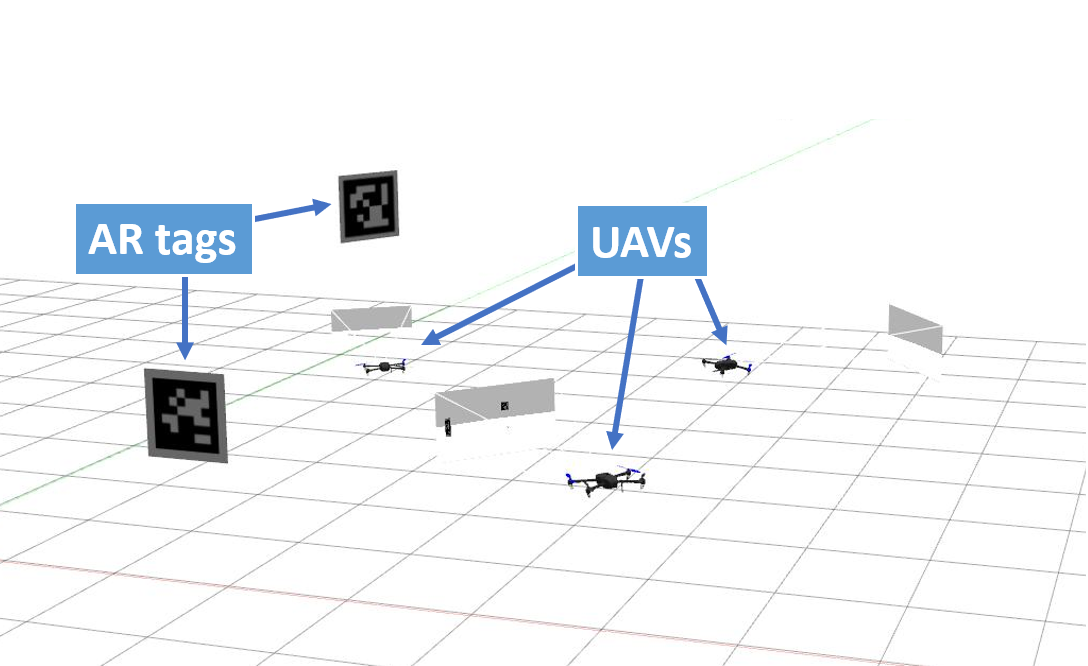
\includegraphics[width=0.65\textwidth]{gazebo-env-1.png}}
\caption{
Gazebo simulation with 3 UAVs and 2 objects (AR Tags) in a 3D Environment.
The UAV can project a viewing frustum to observe the search space.
% A tuple $(e,t)$ represents a pair of space size and number of targets (AR Tags) for search.
% For example, $(8,4)$ stands for the size of $8^3$ with {\color{magenta}2} targets within this environment.
% The red cube represents the robot searching for the target.
}
\label{environment}
\end{figure}

\section{Experiment Setup}
Three experiments are conducted: the target search experiment (EX1), the parametric analysis (EX2), and the scalability analysis (EX3).

In the target search experiment (EX1), the performance of the proposed algorithms (MRSM) is assessed through simulation
(see Fig.~\ref{environment}) and a realistic environment (see Fig.~\ref{GEB_fig}).
The assessment includes a comparison with state-of-the-art approaches (e.g., MRSIS \cite{li2024mrsis}, CapAM \cite{paull2022learning} and PD-FAC \cite{sheng2022pd}).
The simulation is carried out with 3 robots (UAVs) on Gazebo (see Fig. \ref{environment}). Various environment sizes $\mathit{\mathbb{E}}=\{8,12\}$ and numbers of targets (AR tags) $\mathit{\mathbb{T}}=\{2,4,6\}$ in the space are evaluated.
Each $(a,b)$ pair generates 100 trials with randomly located targets,
where $a \in \mathit{\mathbb{E}}$ is an $a \times a \times a (m.)$ search space, and $b \in \mathit{\mathbb{T}}$ is the number of targets in $a$.
The robot's goal is to find all targets in scenarios of partial occlusion.

A weighted graph $\mathcal{G}=(\mathcal{V}, \mathcal{E}, c)$ is constructed to represent the environment, where $\mathcal{V}$ is the subgoal set, $\mathcal{E}$ is the edge set, and $c$ is the routing costs with respect to edges.
The subgoals $\mathcal{V}$ are evenly distributed throughout the space and each subgoal is defined as $v\in \{(x,y,z,\theta)|(x,y,z,\theta)\in \mathcal{V}\}$, where $x,y,z\in[1, e]$ and $\theta\in\{0,60,120,180,240,300\}$.

In the search process, each robot can take one of the actions from $\mathcal{A}=\{Move(x,y,z,\theta), Detect\}$.
The $Move$ action takes the drone to the coordinate $(x,y,z)$ with the heading $\theta$.
The $Detect$ action performs an object detection.
The time constraint of the search process is 10 minutes.
Once all the targets have been found or the search time exceeds the constraint, the task is terminated.

The coverage function ($f$) is calculated by the ratio of the number of covered voxels to the total number of environmental voxels. The routing cost ($c$) is measured by the Euclidean distance between two subgoals\footnote{For any two connected nodes, $v_1=(x_1,y_1,z_1, \theta_1)$ and $v_2=(x_2,y_2,z_2,\theta_2)$, the routing cost $c(\{(v_1,v_2)\})=\sqrt{(x_1-x_2)^2+(y_1-y_2)^2+(z_1-z_2)^2+(\theta_1-\theta_2)^2}$.}.

There are two real-world experiments with 2 drones.
The first one is in a 13 $\times$ 9 $\times$ 2 $m$ public area on the third floor of the General Education Building at the National Central University (NCU) (see Fig. \ref{GEB_fig}(a)).
The space is divided into voxels whose unit size is $15 \times 15 \times 15$ $cm$.
The goal is to find a sports ball, a chair, and a bottle in the environment, shown in Fig. \ref{GEB_fig}(b).
Three targets are randomly located and can be partially occluded due to the complex environment with obstacles.
The second one is in a 50 $\times$ 50 $\times$ 5 $m$ Hengshan Calligraphy Art Park (see Fig. \ref{Call_fig}(a)).
The space contains plenty of obstacles (trees). The goal is to find three AR tags in the environment, shown in Fig. \ref{Call_fig}(b).

The searchers are the drones developed by Taiwan Drone 100 shown in Fig. \ref{drone}.
The drone is equipped with NVIDIA Jetson Xavier NX and two Intel RealSense cameras.
The Intel RealSense T265 camera is used to localize the drone and the D435i camera is to explore the environment.
The camera and drone parameters are shown in Table \ref{Tab:parameters}.

To detect objects, the YOLOv5 \cite{glenn_jocher_2022_7347926} is adopted and run on NVIDIA Jetson Xavier NX.
The uncertainty of detection is considered due to object occlusion in the environment. To successfully detect the object, the confidence rate of detection must be over a threshold of 0.6.

In the parametric analysis experiment (EX2), the parameters, the weight of the balancing function ($\lambda$), and the robot routing budget ($l_i$) are investigated for MRSIS \cite{li2024mrsis} and MRSM algorithms within an $8\times8\times8 (m.)$ simulated environment.
Three robots (UAVs) are tasked to find various numbers of targets $b \in \{2,4,6\}$ with different balancing weights $\lambda\in\{0\,,0.2,\,0.4,\,0.6,\,0.8,\,1\}$ and robot routing budgets $l_i\in\{20,\, 40,\, 60,\, 80\}$.
When $\lambda=0$, no balanced workloads are considered.
When $\lambda=1$, the workloads assigned to robots are thoroughly optimized.
The experiment setup is the same as the simulation in EX1.
Additionally, a comparative analysis of computational time is conducted for both methods.

In the scalability analysis experiment (EX3), the performance of MRSM and MRSIS\cite{li2024mrsis} is evaluated under a
$20\times20\times20(m^3)$ simulated space involving a considerable number of robots $R=\{5, 10\}$.
Performance is evaluated on different numbers of subgoals $\mathcal{V}=\{700,800,900\}$.
Robots (UAVs) must find 8 targets (AR tags) in the environment.
The balancing weight $\lambda$ and robot routing budget $l_i$ are set to $0.2$ and $300$, respectively.
The camera range is set to 5 meters and the remaining configurations are established in the same manner as the simulation in EX1.

Two baseline methods (CapAM\cite{paull2022learning} and PD-FAC\cite{sheng2022pd}) are implemented for the search scenarios. In CapAM\cite{paull2022learning}, the state space of the MDP contains features such as the elapsed mission time, the robot's current location, and the robot's work capacity. The action space of the MDP is the action set $\mathcal{A}$. The goal of CapAM\cite{paull2022learning} is to visit as many subgoals as possible.
In PD-FAC\cite{sheng2022pd}, the weighted graph $\mathcal{G}$ maintains the same format as detailed in \cite{sheng2022pd}. The search time budget is set to 10 minutes and the search targets are randomly placed on the graph nodes. Once the robot visits the node on the graph, the target is marked as found. The configurations of PD-FAC can be found in \cite{sheng2022pd}.

\renewcommand{\arraystretch}{1.3}
\begin{table}[h]
\caption{Parameters of EX1 and EX2.}
\begin{center}
\begin{tabular}{|c||c|c|c|}
\hline
Parameters & Simulation & Real-world search \\
\hline\hline
Camera range & $2m$ & $3m$  \\
\hline
Horizontal FOV & $45^{\circ}$ & $69^{\circ}$  \\
\hline
Vertical FOV & $45^{\circ}$ & $42^{\circ}$ \\
\hline
Transitional velocity & $1.3$ $m/sec$ & $0.2$ $m/sec$ \\
\hline
Angular velocity & $45$ $deg/sec$ & $120$ $deg/sec$ \\
\hline
\end{tabular}
\label{Tab:parameters}
\end{center}
\end{table}


\begin{figure}
    \centering
    \begin{subfigure}[b]{0.5\textwidth}
        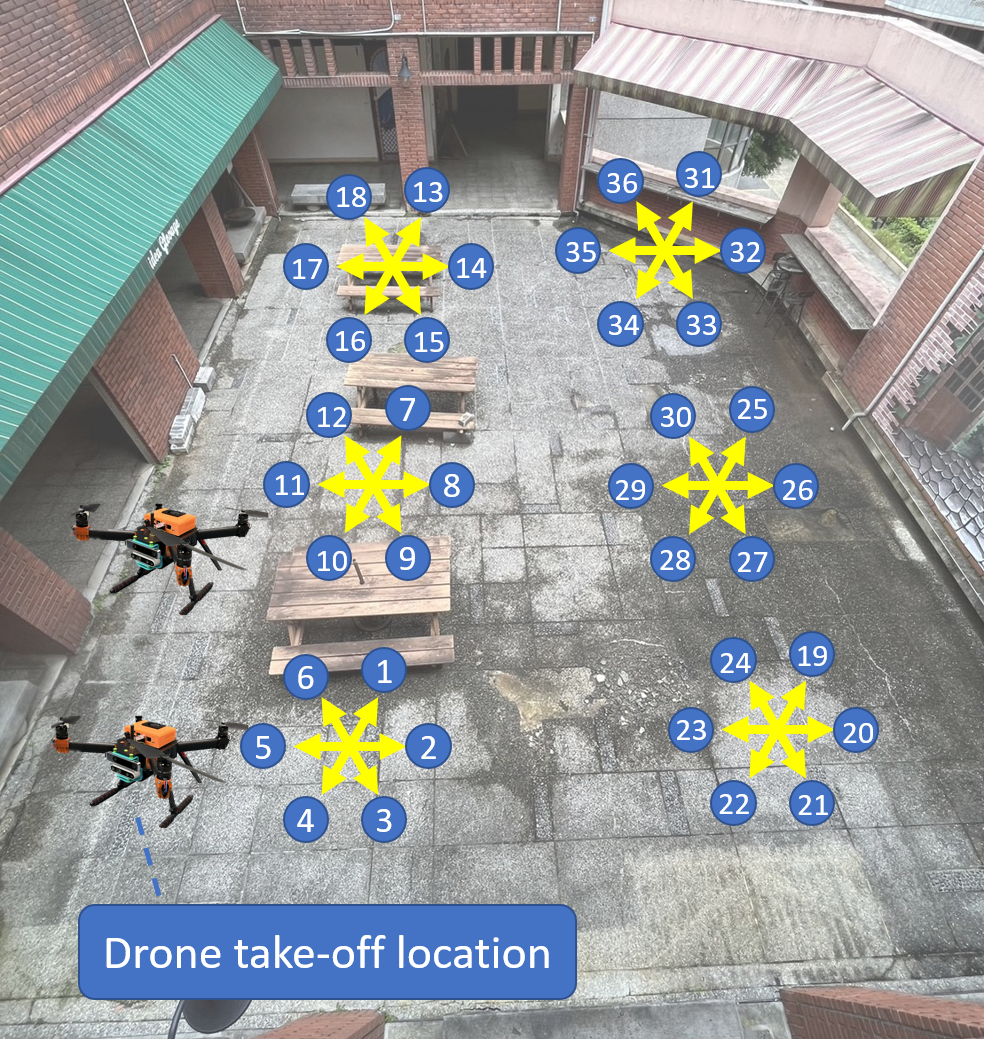
\includegraphics[width=1\textwidth]{GEB.png}
        \caption{} \label{GEB map}
    \end{subfigure}
    \begin{subfigure}[b]{0.5\textwidth}
    \centering
        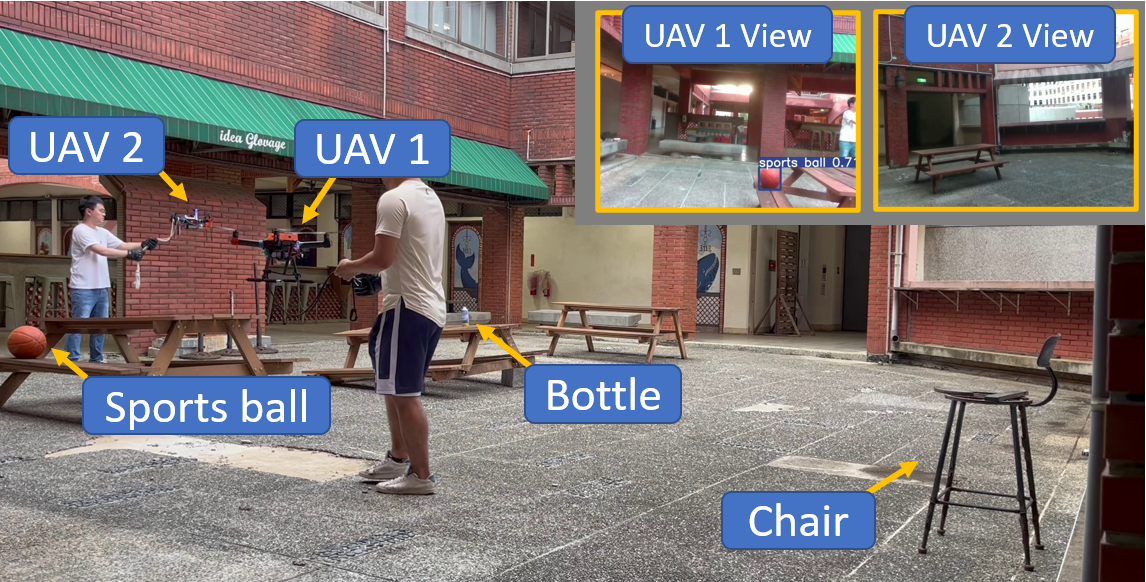
\includegraphics[width=1\textwidth]{exp.png}
        \caption{} \label{GEB exp}
    \end{subfigure}
    \hfill
    \caption{(a) A 13$\times$9 $m.$ public area on the third floor of the General Education Building at the National Central University. (b) An example of UAVs searching for targets (a sports ball, a bottle, and a chair).
    }
    \label{GEB_fig}
\end{figure}

\begin{figure}
  \centering
  \begin{subfigure}[b]{0.21\textwidth}
      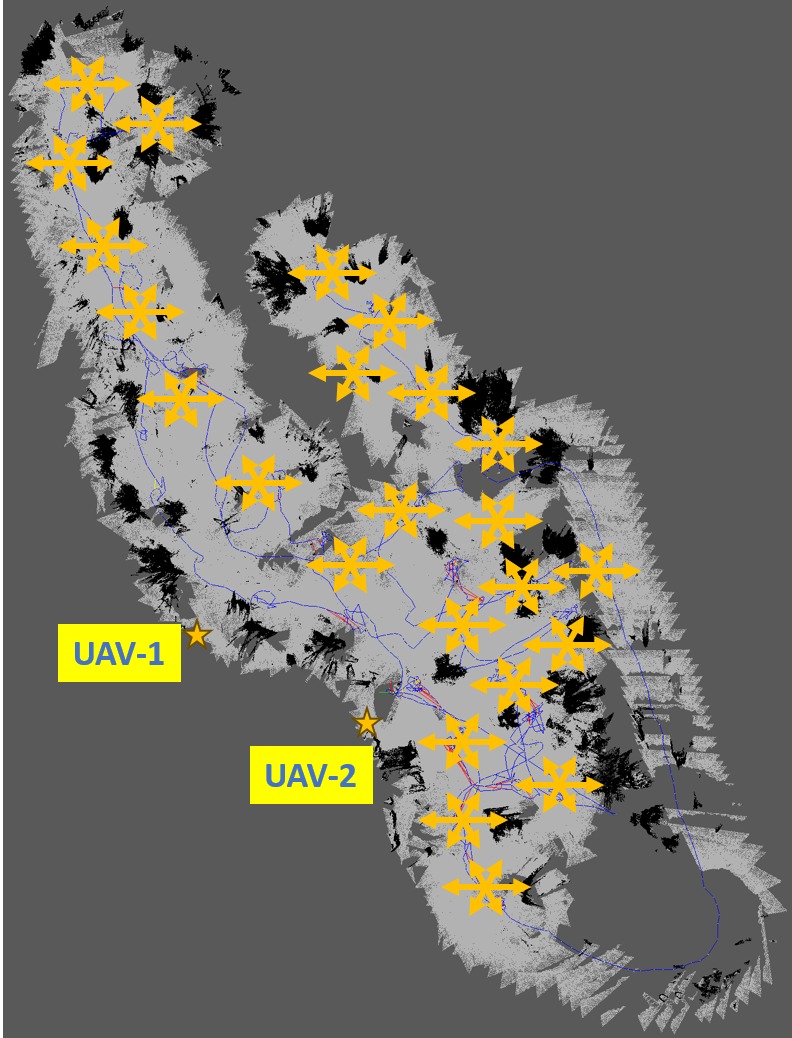
\includegraphics[width=1\textwidth]{map_call.png}
      \caption{} \label{Call map}
  \end{subfigure}
  \begin{subfigure}[b]{0.26\textwidth}
  \centering
      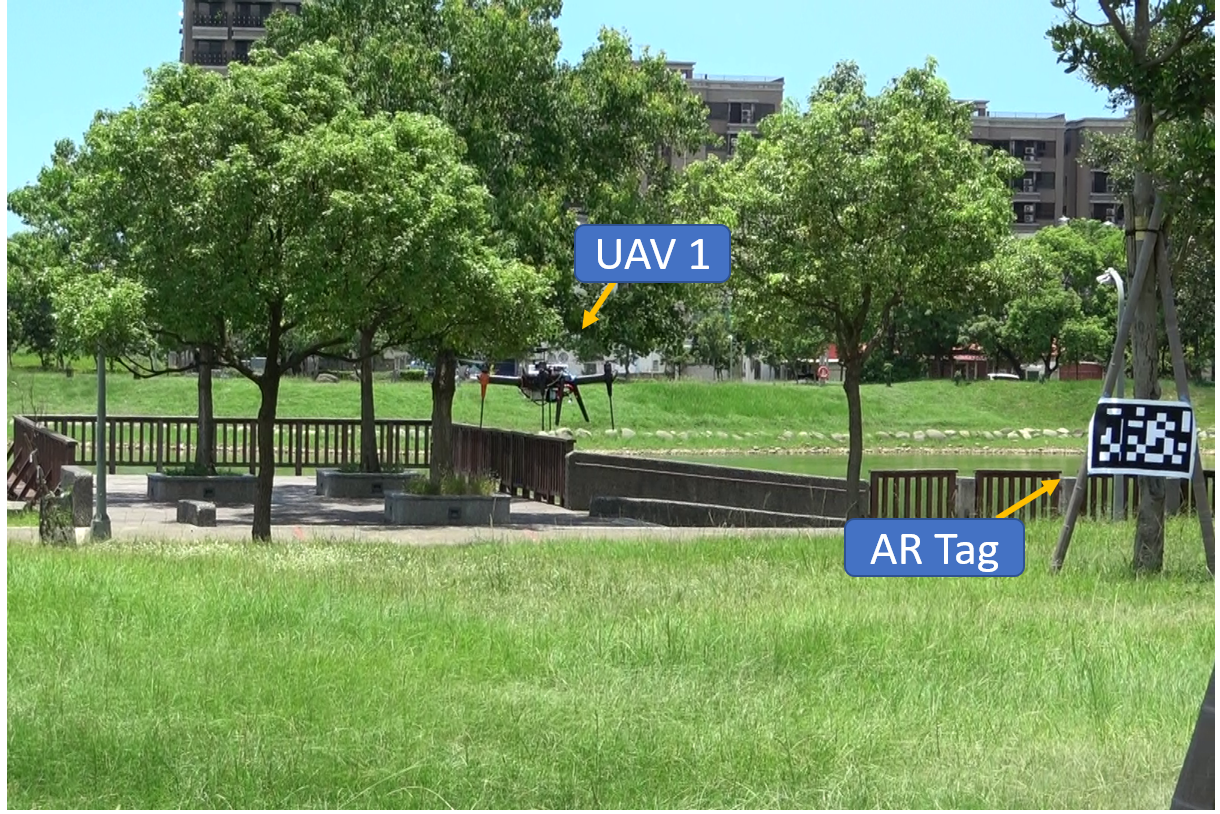
\includegraphics[width=1\textwidth]{Call_uav.png}
      \caption{} \label{Call exp}
  \end{subfigure}
  \hfill
  \caption{(a) A 50$\times$50$\times$5 $m$ lawn at the Hengshan Calligraphy Art Park. (b) An example of a drone searching for AR tags.
  }
  \label{Call_fig}
\end{figure}

\begin{figure}[htbp]
\centerline{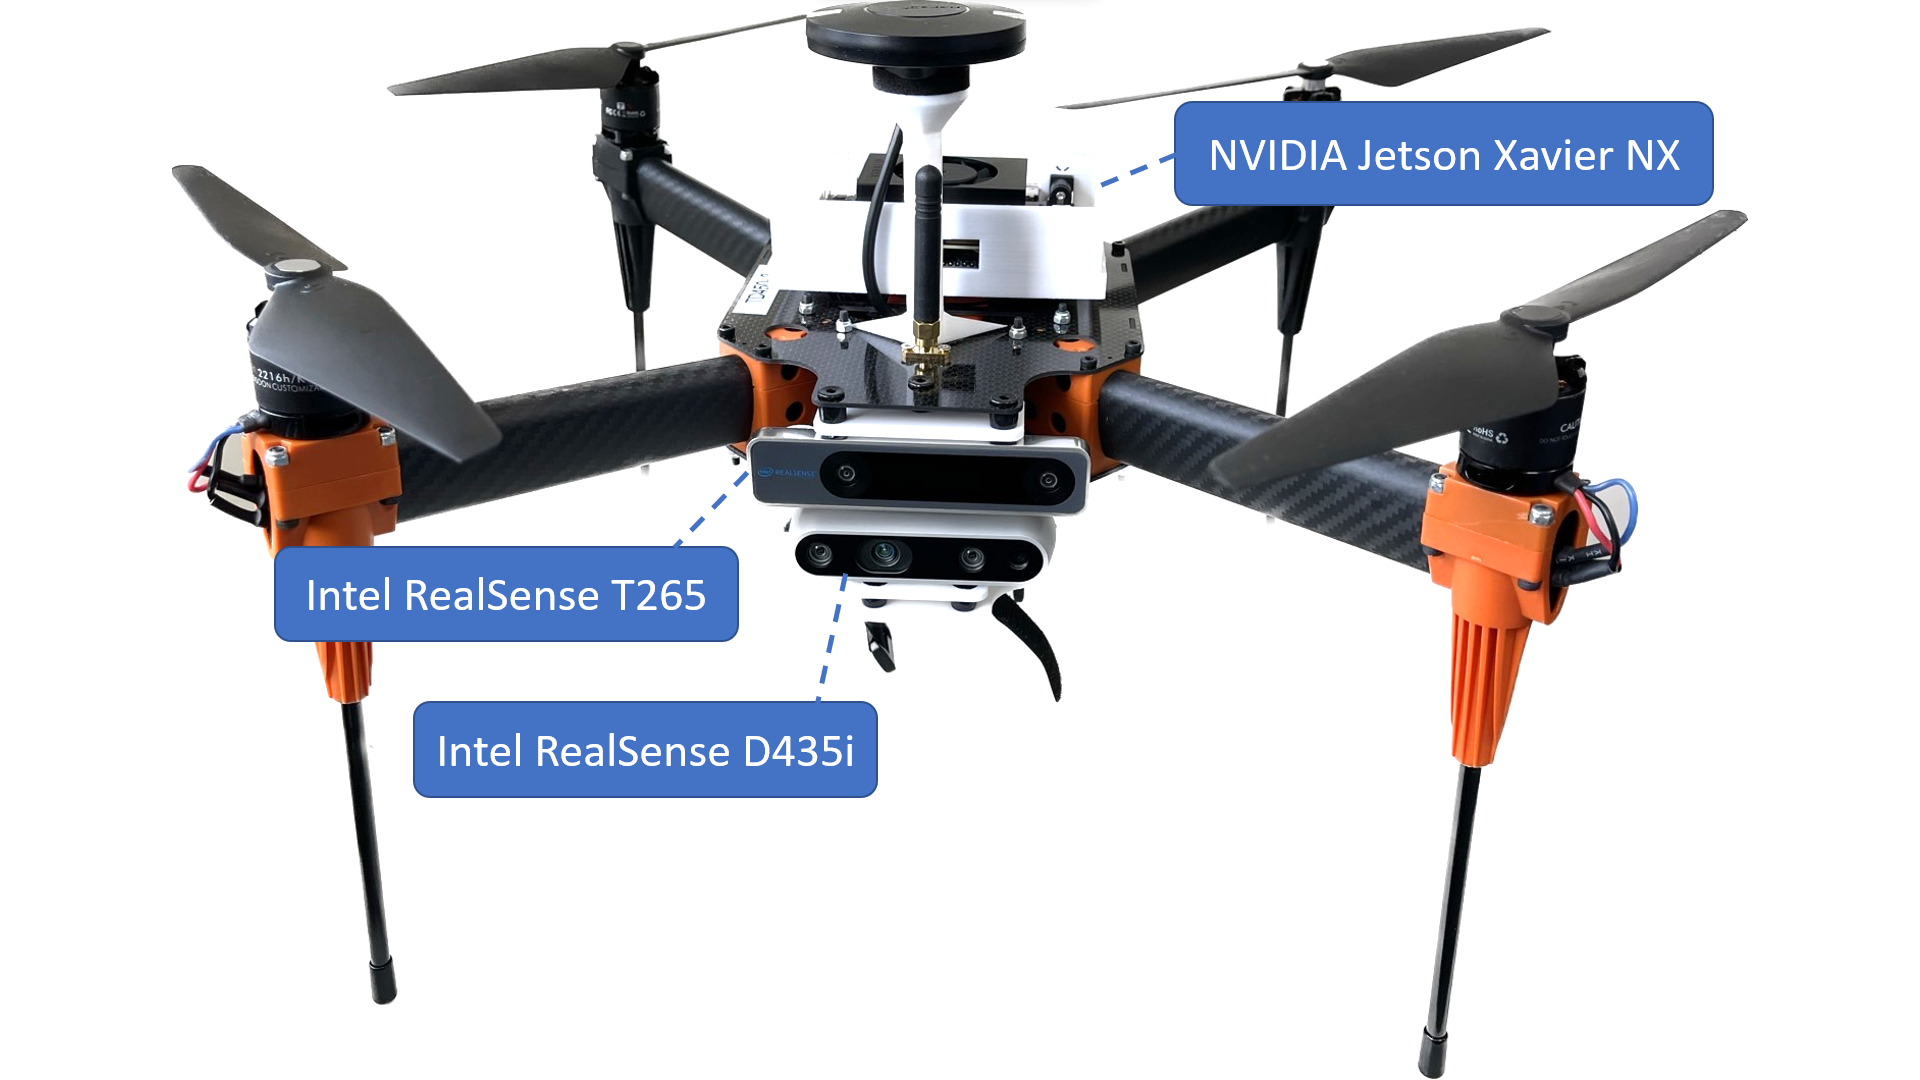
\includegraphics[width=0.6\textwidth]{uav.png}}
\caption{A customized UAV developed by Taiwan Drone 100.}
\label{drone}
\end{figure}

\section{EX$1$: Comparison with Benchmarks on Targets Search}
Table \ref{tab:ANDO} and Table \ref{tab:ETTD} present the simulated performance with a routing budget $l_i=350$, the number of robots $k=3$ and a balancing function weight $\lambda=1$ across various environment sizes.
MRSM is compared to state-of-the-art baselines (e.g., MRSIS\cite{li2024mrsis}, CapAM\cite{paull2022learning}, AM-RL\cite{kool2018attention}, and PD-FAC\cite{sheng2022pd}).

In Table \ref{tab:ANDO}, drones find more objects in a small environment ($a=8$) compared to the larger one ($a=12$).
The decrease in the number of targets in the environment correlates with an increase in the difficulty of the search.
MRSM achieves the highest ENDO in the large environment ($a=12$).
The advantage of MRSM lies in its ability to maximize both the coverage function and the workload balancing function under matroid constraints.
In addition, MRSIS-TSP and MRSM performance is very close in the case of $a=8$. The detailed performance of both MRSM and MRSIS-TSP \cite{li2024mrsis} will be examined in EX2.

Table \ref{tab:ETTD} shows the ETTD of all methods.
All approaches are constrained to search within 10 minutes (600 seconds).
For $a=8$, MRSIS-MST \cite{li2024mrsis} is the most efficient, while for $a=12$, MRSM takes the lead in efficiency.
MRSM, in comparison to AM-RL \cite{kool2018attention}, detects fewer average targets in the $a=8$ scenario.
Despite AM-RL \cite{kool2018attention} finding the highest ENDO, especially within the time constraint of 600 seconds, its search efficiency is compromised due to the largest ETTD value.

To further examine the proposed approaches, algorithms (MRSIS\cite{li2024mrsis}, CapAM\cite{paull2022learning}, and PD-FAC\cite{sheng2022pd}) are evaluated in a real-world environment. Experiments are conducted 5 times for each approach.

In the National Central University scenario, the ETTD and the coverage rate are shown in Table \ref{ETTD table in GEB}.
MRSM achieves an ETTD of 201 seconds and a coverage rate of 67\%, which is the lowest ETTD and the highest coverage rate among other approaches.
Unlike the MST approach (MRSIS-MST \cite{li2024mrsis}), MRSM generates spanning trees that may not be the shortest trajectories, but are the most efficient for target discovery.
The experiments demonstrate that MRSM outperforms benchmark algorithms. In the Hengshan Calligraphy Art Park environment, the ETTD and the coverage rate are shown in Table \ref{ETTD table in Calligraphy}. MRSM outperforms the benchmarks in ETTD, achieving an ETTD of 196 seconds and a coverage rate of 31\%.

The summaries of these experiments are as follows.
The proposed algorithm (MRSM) outperforms state-of-the-art approaches (e.g., MRSIS\cite{li2024mrsis}, AM-RL\cite{kool2018attention}, CapAM\cite{paull2022learning}, and PD-FAC\cite{sheng2022pd}) as claimed in Thm. \ref{def:proposed-bound}.
MRSM achieves the highest coverage rate and discovers targets with the lowest ETTD.
However, it is not guaranteed to find the most targets in the environment.


\begin{table}[h]
  \centering
  \caption{The expected number of detected objects (ENDO) in various environment sizes ($\mathit{\mathbb{E}}$) and number of targets ($\mathit{\mathbb{T}}$) on Gazebo simulator.}
  \label{tab:ANDO}
  \begin{tabular}{ccccccc}
  \toprule
   $\mathit{\mathbb{E}}$ & \multicolumn{3}{c}{8} & \multicolumn{3}{c}{12} \\
  \cmidrule(lr){2-4} \cmidrule(lr){5-7}
   $\mathit{\mathbb{T}}$ & 2 & 4 & 6 & 2 & 4 & 6 \\
  \midrule
  Random & 0.86 & 1.43 & 2.25 & 0.12 & 0.34 & 0.52 \\
  AM-RL & \textbf{1.5} & \textbf{3.15} & \textbf{4.73} & 0.23 & 0.56 & 0.77 \\
  CapAM & 0.89 & 1.69 & 2.48 & 0.34 & 0.81 & 1.18 \\
  PD-FAC & 0.49 & 0.81 & 1.11 & 0.15 & 0.43 & 0.46 \\
  MRSIS-MST & 1.03 & 2.14 & 3.21 & 0.51 & 0.99 & 1.51 \\
  MRSIS-TSP & 1.46 & 2.92 & 4.41 & 1.60 & 3.01 & 4.88 \\
  MRSM & 1.44 & 2.92 & 4.39 & \textbf{1.68} & \textbf{3.19} & \textbf{4.97} \\
  \bottomrule
  \end{tabular}
  \end{table}

  \begin{table}[h]
    \centering
    \caption{The ETTD in various environment sizes ($\mathit{\mathbb{E}}$) and number of targets ($\mathit{\mathbb{T}}$) on Gazebo simulator. The unit is seconds.}
    \label{tab:ETTD}
    \begin{tabular}{ccccccc}
    \toprule
    $\mathit{\mathbb{E}}$ & \multicolumn{3}{c}{$8$} & \multicolumn{3}{c}{$12$} \\
    \cmidrule(lr){2-4} \cmidrule(lr){5-7}
    $\mathit{\mathbb{T}}$ & $2$ & $4$ & $6$ & $2$ & $4$ & $6$ \\
    \midrule
    Random    & $480$ & $438$ & $428$ & $600$ & $600$ & $600$ \\
    AM-RL     & $600$ & $600$ & $600$ & $565$ & $540$ & $518$ \\
    CapAM     & $463$ & $418$ & $377$ & $544$ & $500$ & $463$ \\
    PD-FAC    & $525$ & $450$ & $439$ & $556$ & $497$ & $486$ \\
    MRSIS-MST & $\mathbf{251}$ & $\mathbf{211}$ & $\mathbf{205}$ & $532$ & $478$ & $454$ \\
    MRSIS-TSP & $264$ & $273$ & $259$ & $379$ & $416$ & $386$ \\
    MRSM      & $260$ & $271$ & $258$ & $\mathbf{365}$ & $\mathbf{392}$ & $\mathbf{368}$ \\
    \bottomrule
    \end{tabular}
    \end{table}


\begin{table}[h]
  \centering
  \caption{The ETTD of MRSM and baselines (MRSIS \cite{li2024mrsis}, CapAM \cite{paull2022learning}, and PD-FAC \cite{sheng2022pd}) at the National Central University.}
  \label{ETTD table in GEB}
  \begin{tabular}{cccc}
  \toprule
  Method         & Mean (sec.) & Std. & Coverage Rate \\
  \midrule
  CapAM          & $275$       & $93$ & $42\%$ \\
  PD-FAC         & $314$       & $130$ & $33\%$ \\
  MRSIS-MST      & $206$       & $75$  & $65\%$ \\
  MRSIS-TSP      & $280$       & $58$  & $62\%$ \\
  MRSM           & $\mathbf{201}$ & $93$  & $\mathbf{67\%}$ \\
  \bottomrule
  \end{tabular}
\end{table}

\begin{table}[h]
  \centering
  \caption{The ETTD of MRSM and baselines (MRSIS \cite{li2024mrsis}, CapAM \cite{paull2022learning}, and PD-FAC \cite{sheng2022pd}) at the Hengshan Calligraphy Art Park.}
  \label{ETTD table in Calligraphy}
  \begin{tabular}{cccc}
  \toprule
  Method         & Mean (sec.) & Std. & Coverage Rate \\
  \midrule
  CapAM          & $299$       & $63$ & $22\%$ \\
  PD-FAC         & $268$       & $55$ & $27\%$ \\
  % MRSIS-MST      & $206$       & $75$  & $65\%$ \\
  % MRSIS-TSP      & $280$       & $58$  & $62\%$ \\
  MRSM           & $\mathbf{196}$ & $31$  & $\mathbf{31\%}$ \\
  \bottomrule
  \end{tabular}
\end{table}

%\clearpage
\begin{figure}
   \centering
   \begin{subfigure}[b]{0.45\textwidth}
       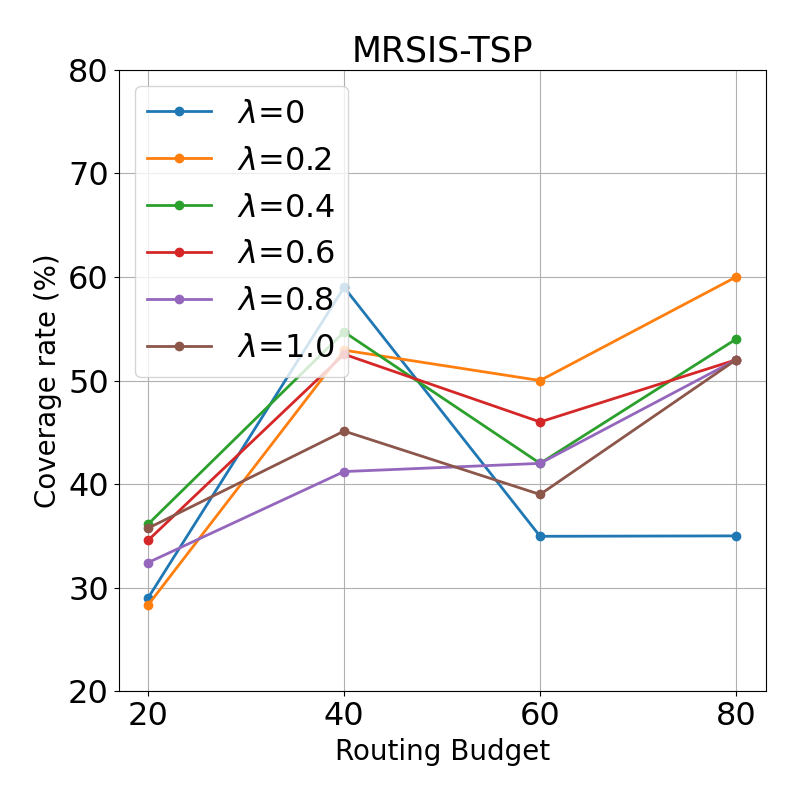
\includegraphics[width=1\textwidth]{MRSIS-TSP-cov.png}
       \caption{MRSIS-TSP\cite{li2024mrsis}}
   \end{subfigure}
   \hfill
   \quad
   \centering
   \begin{subfigure}[b]{0.45\textwidth}
       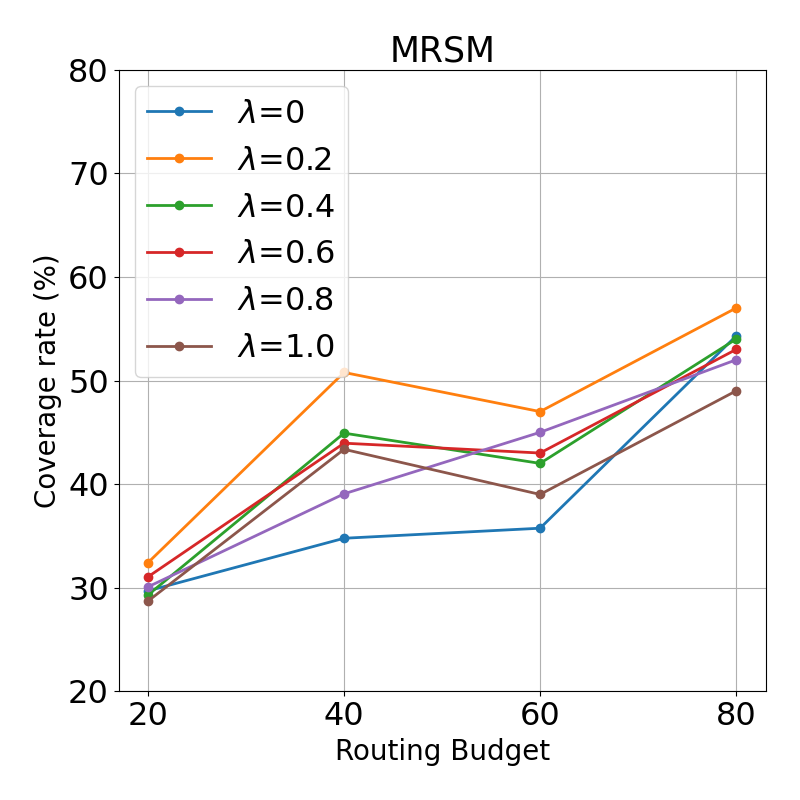
\includegraphics[width=1\textwidth]{MRSM-cov.png}
       \caption{MRSM}
   \end{subfigure}
   \hfill
   \caption{Coverage rate with different robot routing budget $l_i$ and balancing weight $\lambda$.}
   \label{fig:lbd-cov}
\end{figure}

\begin{figure}
   \centering
   \begin{subfigure}[b]{0.45\textwidth}
       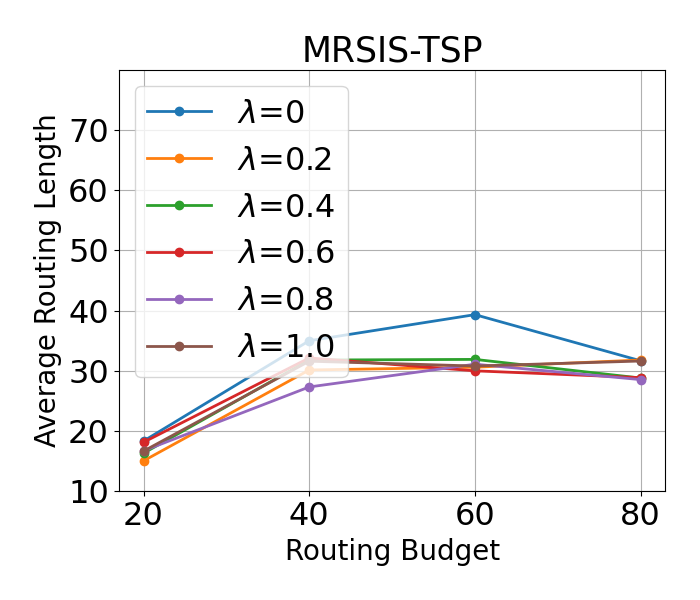
\includegraphics[width=1\textwidth]{MRSIS-TSP.png}
       \caption{MRSIS-TSP\cite{li2024mrsis}}
   \end{subfigure}
   \hfill
   \quad
   \centering
   \begin{subfigure}[b]{0.45\textwidth}
       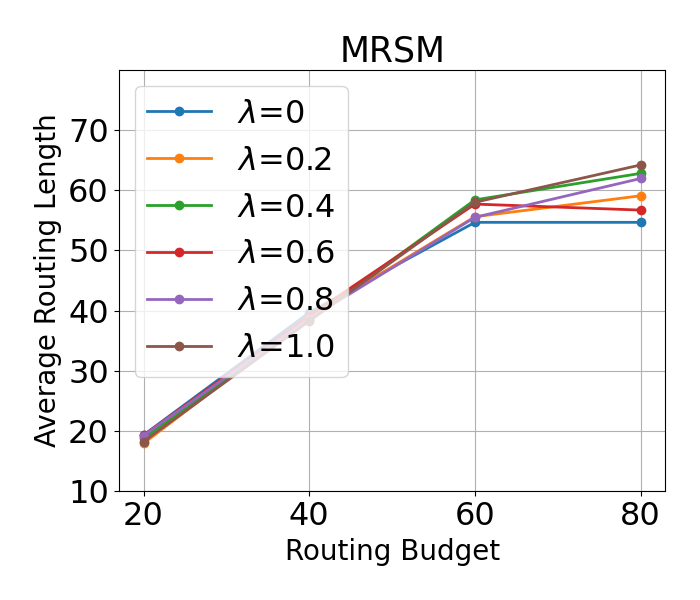
\includegraphics[width=1\textwidth]{MRSM.png}
       \caption{MRSM}
   \end{subfigure}
   \hfill
   \caption{Average routing length (in meters) with various balancing weights $\lambda$ and robot routing budget.}
   \label{fig:routing}
\end{figure}

\begin{table}[h]
  \centering
  \caption{The expected number of detected objects (ENDO) with different parameters (robot routing budget $l_i$, number of targets $b$, and balancing weight $\lambda$) on Gazebo simulator.}
  \label{tab:ANDO-lambda}
  \resizebox{0.6\textwidth}{!}{%
  \begin{tabular}{cccccccccc}
  \toprule
  \multirow{2}{*}{$l_i$} & \multirow{2}{*}{$b$} & \multirow{2}{*}{Method} & \multicolumn{6}{c}{$\lambda$} \\
  \cmidrule(lr){4-9}
   &  &  & 0 & 0.2 & 0.4 & 0.6 & 0.8 & 1 \\
  \midrule
  \multirow{6}{*}{20} & \multirow{2}{*}{2} & MRSIS-TSP & 0.8 & 1.0 & 1.1 & 1.0 & 1.1 & 1.1 \\
   &  & MRSM & \textbf{1.1} & \textbf{1.1} & \textbf{1.2} & \textbf{1.2} & \textbf{1.1} & \textbf{1.1} \\
  \cmidrule(lr){2-9}
   & \multirow{2}{*}{4} & MRSIS-TSP & 1.8 & 2.1 & 2.3 & 2.3 & 2.2 & 2.0 \\
   &  & MRSM & \textbf{2.3} & \textbf{2.2} & \textbf{2.3} & \textbf{2.4} & \textbf{2.2} & \textbf{2.2} \\
  \cmidrule(lr){2-9}
   & \multirow{2}{*}{6} & MRSIS-TSP & 2.6 & 3.2 & 3.4 & 3.4 & 3.2 & 3.1 \\
   &  & MRSM & \textbf{3.4} & \textbf{3.3} & \textbf{3.4} & \textbf{3.6} & \textbf{3.2} & \textbf{3.3} \\
  \midrule
  \multirow{6}{*}{40} & \multirow{2}{*}{2} & MRSIS-TSP & \textbf{1.5} & 1.3 & 1.4 & 1.4 & 1.2 & \textbf{1.5} \\
   &  & MRSM & 1.2 & \textbf{1.4} & \textbf{1.4} & \textbf{1.4} & \textbf{1.3} & 1.3 \\
  \cmidrule(lr){2-9}
   & \multirow{2}{*}{4} & MRSIS-TSP & \textbf{3.2} & 2.8 & 2.8 & \textbf{3.1} & 2.6 & \textbf{3.0} \\
   &  & MRSM & 2.4 & \textbf{2.9} & \textbf{2.8} & 2.9 & \textbf{2.7} & 2.8 \\
  \cmidrule(lr){2-9}
   & \multirow{2}{*}{6} & MRSIS-TSP & \textbf{4.6} & 4.1 & 4.2 & \textbf{4.5} & 3.8 & \textbf{4.5} \\
   &  & MRSM & 3.5 & \textbf{4.5} & \textbf{4.3} & 4.3 & \textbf{4.1} & 4.1 \\
  \midrule
  \multirow{6}{*}{60} & \multirow{2}{*}{2} & MRSIS-TSP & \textbf{1.3} & \textbf{1.0} & \textbf{1.0} & \textbf{1.0} & \textbf{1.0} & \textbf{1.0} \\
   &  & MRSM & 1.3 & 0.9 & 0.9 & 0.9 & 0.9 & 0.9 \\
  \cmidrule(lr){2-9}
   & \multirow{2}{*}{4} & MRSIS-TSP & 2.6 & \textbf{2.2} & \textbf{2.0} & \textbf{2.2} & \textbf{2.2} & \textbf{2.1} \\
   &  & MRSM & \textbf{2.7} & 2.1 & 1.9 & 2.0 & 2.0 & 1.8 \\
  \cmidrule(lr){2-9}
   & \multirow{2}{*}{6} & MRSIS-TSP & 3.7 & \textbf{3.3} & \textbf{3.0} & \textbf{3.2} & \textbf{3.3} & \textbf{3.2} \\
   &  & MRSM & \textbf{4.0} & 3.1 & 2.9 & 2.9 & 3 & 2.8 \\
  \midrule
  \multirow{6}{*}{80} & \multirow{2}{*}{2} & MRSIS-TSP & 1.3 & \textbf{1.5} & \textbf{1.5} & 1.4 & \textbf{1.4} & \textbf{1.4} \\
   &  & MRSM & \textbf{1.5} & 1.4 & 1.5 & \textbf{1.5} & 1.4 & 1.4 \\
  \cmidrule(lr){2-9}
   & \multirow{2}{*}{4} & MRSIS-TSP & 2.7 & \textbf{3.2} & \textbf{3.0} & 2.8 & 2.9 & \textbf{3.1} \\
   &  & MRSM & \textbf{3.1} & 3.1 & 3.0 & \textbf{3.1} & \textbf{3.0} & 2.9 \\
  \cmidrule(lr){2-9}
   & \multirow{2}{*}{6} & MRSIS-TSP & 4 & \textbf{4.6} & \textbf{4.4} & 4.1 & 4.3 & \textbf{4.4} \\
   &  & MRSM & \textbf{4.7} & 4.4 & 4.4 & \textbf{4.5} & \textbf{4.4} & 4.3 \\
  \bottomrule
  \end{tabular} }
  \end{table}


  \begin{table}[h]
  \centering
  \caption{The ETTD with different parameters (robot routing budget $l_i$, number of targets $b$, and balancing weight $\lambda$) on Gazebo simulator. The unit is in seconds.}
  \label{tab:ETTD-lambda}
  \resizebox{0.6\textwidth}{!}{%
  \begin{tabular}{ccccccccc}
  \hline
  \multirow{2}{*}{$l_i$} & \multirow{2}{*}{$b$} & \multirow{2}{*}{Method} & \multicolumn{6}{c}{$\lambda$} \\ \cline{4-9}
   &  &  & 0 & 0.2 & 0.4 & 0.6 & 0.8 & 1 \\ \hline
  \multirow{6}{*}{20} & \multirow{2}{*}{2} & MRSIS-TSP & 384 & 342 & 335 & 347 & 328 & 342 \\
   &  & MRSM & \textbf{326} & \textbf{315} & \textbf{303} & \textbf{282} & \textbf{323} & \textbf{328} \\ \cline{2-9}
   & \multirow{2}{*}{4} & MRSIS-TSP & 382 & 340 & \textbf{313} & 325 & 337 & 355 \\
   &  & MRSM & \textbf{308} & \textbf{313} & 315 & \textbf{292} & \textbf{317} & \textbf{328} \\ \cline{2-9}
   & \multirow{2}{*}{6} & MRSIS-TSP & 378 & 334 & \textbf{313} & 316 & 330 & 348 \\
   &  & MRSM & \textbf{309} & \textbf{313} & 314 & \textbf{292} & \textbf{327} & 320 \\ \hline
  \multirow{6}{*}{40} & \multirow{2}{*}{2} & MRSIS-TSP & \textbf{272} & 302 & 282 & 271 & 316 & \textbf{258} \\
   &  & MRSM & 309 & \textbf{261} & \textbf{278} & \textbf{261} & \textbf{293} & 300 \\ \cline{2-9}
   & \multirow{2}{*}{4} & MRSIS-TSP & \textbf{251} & 275 & 289 & \textbf{249} & 292 & \textbf{261} \\
   &  & MRSM & 329 & \textbf{264} & \textbf{286} & 252 & \textbf{279} & 273 \\ \cline{2-9}
   & \multirow{2}{*}{6} & MRSIS-TSP & \textbf{260} & 278 & 277 & 249 & 292 & \textbf{247} \\
   &  & MRSM & 320 & \textbf{246} & \textbf{255} & \textbf{244} & \textbf{277} & 269 \\ \hline
  \multirow{6}{*}{60} & \multirow{2}{*}{2} & MRSIS-TSP & \textbf{307} & \textbf{266} & \textbf{270} & \textbf{283} & \textbf{266} & \textbf{297} \\
   &  & MRSM & 308 & 317 & 318 & 307 & 324 & 328 \\ \cline{2-9}
   & \multirow{2}{*}{4} & MRSIS-TSP & \textbf{310} & \textbf{195} & \textbf{203} & \textbf{223} & \textbf{205} & \textbf{226} \\
   &  & MRSM & 312 & 229 & 271 & 243 & 238 & 249 \\ \cline{2-9}
   & \multirow{2}{*}{6} & MRSIS-TSP & 321 & \textbf{159} & \textbf{158} & \textbf{190} & \textbf{148} & \textbf{179} \\
   &  & MRSM & \textbf{301} & 205 & 231 & 194 & 209 & 204 \\ \hline
  \multirow{6}{*}{80} & \multirow{2}{*}{2} & MRSIS-TSP & 313 & \textbf{277} & \textbf{273} & 286 & \textbf{275} & \textbf{263} \\
   &  & MRSM & \textbf{269} & 288 & 274 & \textbf{273} & 286 & 280 \\ \cline{2-9}
   & \multirow{2}{*}{4} & MRSIS-TSP & 293 & \textbf{256} & \textbf{275} & 288 & \textbf{266} & \textbf{242} \\
   &  & MRSM & \textbf{286} & 257 & 280 & \textbf{267} & 279 & 290 \\ \cline{2-9}
   & \multirow{2}{*}{6} & MRSIS-TSP & 291 & \textbf{260} & 274 & 286 & \textbf{256} & \textbf{249} \\
   &  & MRSM & \textbf{271} & 270 & \textbf{271} & \textbf{262} & 269 & 278 \\ \hline
  \end{tabular} }
  \end{table}


  \begin{table}[]
    \centering
    \caption{The ENDO of MRSM with different parameters (environment sizes $\mathbb{E}$, number of targets $b$, and balancing weights $\lambda$) on Gazebo simulator.}
    \label{tab:ENDO-Env-lambda}
    \begin{tabular}{ccllllll}
    \hline
    \multirow{2}{*}{$\mathbb{E}$} & \multirow{2}{*}{$b$} & \multicolumn{6}{c}{$\lambda$}                                                                 \\ \cline{3-8}
     &
       &
      \multicolumn{1}{c}{0} &
      \multicolumn{1}{c}{0.2} &
      \multicolumn{1}{c}{0.4} &
      \multicolumn{1}{c}{0.6} &
      \multicolumn{1}{c}{0.8} &
      \multicolumn{1}{c}{1} \\ \hline
    \multirow{3}{*}{8} &
      2 &
      1.62 &
      \textbf{1.96} &
      \textbf{1.96} &
      \textbf{1.96} &
      \textbf{1.96} &
      1.91 \\
                         & 4                    & 3.18          & 3.87          & 3.88          & 3.90          & 3.86          & \textbf{3.92} \\
                         & 6                    & 4.91          & 5.90          & \textbf{5.91} & 5.89          & 5.85          & 5.87          \\ \hline
    \multirow{3}{*}{10}  & 2                    & 1.55          & \textbf{1.68} & 1.53          & 1.60          & 1.54          & 1.57          \\
                         & 4                    & 2.80          & 3.19          & 3.16          & 3.23          & 3.06          & \textbf{3.33} \\
                         & 6                    & 4.25          & 4.88          & 4.72          & 4.98          & 4.58          & \textbf{5.04} \\ \hline
    \multirow{3}{*}{12}  & 2                    & 1.02          & 0.92          & 1.09          & 0.97          & 1.08          & \textbf{0.97} \\
                         & 4                    & 1.83          & 1.99          & 2.07          & 1.89          & \textbf{2.25} & 1.74          \\
                         & 6                    & 2.88          & 3.03          & \textbf{3.13} & 2.84          & 2.90          & 2.75          \\ \hline
    \multirow{3}{*}{14}  & 2                    & \textbf{0.68} & 0.62          & 0.58          & 0.61          & 0.64          & 0.54          \\
                         & 4                    & 1.18          & 1.04          & 1.00          & \textbf{1.19} & 1.01          & 1.02          \\
                         & 6                    & 1.65          & 1.77          & 1.62          & \textbf{1.69} & 1.68          & 1.46          \\ \hline
    \end{tabular}
    \end{table}



    \begin{table}[]
    \centering
    \caption{The ETTD of MRSM with different parameters (environment sizes $\mathbb{E}$, number of targets $b$, and balancing weights $\lambda$) on Gazebo simulator. The unit is in seconds.}
    \label{tab:ETTD-Env-lambda}
    \begin{tabular}{ccllllll}
    \hline
    \multirow{2}{*}{$\mathbb{E}$} &
      \multirow{2}{*}{$b$} &
      \multicolumn{6}{c}{$\lambda$} \\ \cline{3-8}
     &
       &
      \multicolumn{1}{c}{0} &
      \multicolumn{1}{c}{0.2} &
      \multicolumn{1}{c}{0.4} &
      \multicolumn{1}{c}{0.6} &
      \multicolumn{1}{c}{0.8} &
      \multicolumn{1}{c}{1} \\ \hline
    \multirow{3}{*}{8}  & 2 & 200          & 125          & 127          & 128          & \textbf{122} & 141          \\
                        & 4 & 207          & 130          & 135          & \textbf{125} & 133          & 131          \\
                        & 6 & 196          & \textbf{121} & 129          & 128          & 129          & 131          \\ \hline
    \multirow{3}{*}{10} & 2 & 217          & \textbf{179} & 212          & 190          & 208          & 209          \\
                        & 4 & 257          & 202          & 198          & 184          & 211          & \textbf{183} \\
                        & 6 & 251          & 195          & 199          & \textbf{173} & 212          & 180          \\ \hline
    \multirow{3}{*}{12} & 2 & 337          & 360          & \textbf{313} & 345          & 320          & 344          \\
                        & 4 & 366          & 340          & 332          & 353          & \textbf{310} & 370          \\
                        & 6 & 354          & 337          & \textbf{329} & 351          & 352          & 357          \\ \hline
    \multirow{3}{*}{14} & 2 & \textbf{420} & 435          & 447          & 440          & 431          & 458          \\
                        & 4 & \textbf{445} & 461          & 468          & \textbf{445} & 468          & 465          \\
                        & 6 & 455          & \textbf{443} & 457          & 451          & 453          & 471          \\ \hline
    \end{tabular}
    \end{table}


\section{EX$2$: Parametric Analysis}
To verify the parametric analysis of MRSIS-TSP\cite{li2024mrsis} and MRSM, the parameters (the coverage rate, the average routing length, the ENDO, and the ETTD) are compared in various balancing weights ($\lambda$) and robot routing budgets ($l_i$).

The coverage rate of MRSIS-TSP\cite{li2024mrsis} and MRSM under different balancing weights ($\lambda$) and robot routing budgets ($l_i$) is as follows.
Fig. \ref{fig:lbd-cov}(a) illustrates the coverage rate of MRSIS-TSP\cite{li2024mrsis}.
When $\lambda=0$, a substantial variance exists among the routing budgets.
No balancing function outperforms at $l_i=40$ while performing less effectively in other cases.
Besides, a smaller balancing weight demonstrates effective performance.
At $l_i=20$, $l_i=60$, and $l_i=80$, a small magnitude of the balancing weight performs optimally.
At $l_i=40$, no balancing function ranks the highest. However, when the balancing function is considered, $\lambda=0.4$ achieves the highest coverage rate.
Fig. \ref{fig:lbd-cov}(b) illustrates the coverage rate of MRSM.
The weight $\lambda=0.2$ yields the highest coverage rate across all routing budget cases.
Besides, the coverage rate of MRSM is more consistent than that of MRSIS-TSP\cite{li2024mrsis}.

Fig. \ref{fig:routing} illustrates the average routing length on 3 robots with various balancing weights ($\lambda$) and robot routing budgets ($l_i$).
As the routing budget increases, robots cover larger traveling distances.
The routing length converges due to the limitation of environment size.
In MRSIS-TSP\cite{li2024mrsis} scenario (Fig. \ref{fig:routing}(a)), robots travel between 10 and 40 meters.
In MRSM scenario (Fig. \ref{fig:routing}(b)), the traveled distance is between 20 and 65 meters.
The reason for the smaller routing distance in MRSIS-TSP\cite{li2024mrsis} compared to MRSM is that MRSIS-TSP\cite{li2024mrsis} utilizes a TSP approximator to minimize travel distances.
Therefore, the average routing length of MRSM is more than that of MRSIS-TSP\cite{li2024mrsis}.

Table \ref{tab:ANDO-lambda} and Table \ref{tab:ETTD-lambda} show the ENDO and the ETTD, respectively.
The best performance is highlighted in bold.
The results indicate that no single method consistently outperforms in all cases.
On average, MRSM outperforms in 38 out of 72 cases, while MRSIS-TSP\cite{li2024mrsis} achieves superiority in 34 out of 72 cases.
Additionally, MRSM excels in small routing budgets ($l_i\leq40$), while MRSIS-TSP\cite{li2024mrsis} performs well in the larger ones.
Since MRSIS-TSP\cite{li2024mrsis} inherits the routing minimization feature, it has an advantage in larger routing budgets by facilitating efficient travel.
Moreover, in some cases, the performance is superior when the balancing function is not involved.
Since the proposed objective function is defined as $F(S)=f(S)+\lambda \mathcal{B}(S)$, when $\lambda=0$, the objective function is simply a coverage function.
Optimizing the coverage function with routing and clustering constraints may yield good performance in certain cases.

To elucidate the use of parameters, Table \ref{tab:ENDO-Env-lambda} and Table \ref{tab:ETTD-Env-lambda} show the performance (ENDO and ETTD) of MRSM in various environment sizes and number of targets. Small environments allow for faster target detection compared to large ones. While no single lambda value is optimal for all environment sizes, empirical results indicate that small environments benefit from larger lambda values, whereas large environments can perform well with smaller lambda values. As the environment size increases, the results suggest that a large area can be covered even with an imbalance in workload distribution.


The EX2 results demonstrate that a small balancing weight magnitude leads to optimal performance for both MRSM and MRSIS-TSP \cite{li2024mrsis}. Across most cases, MRSM outperforms MRSIS-TSP \cite{li2024mrsis} due to the theoretical guarantee of submodularity under matroid constraints. In contrast, smaller environments require a more balanced workload assignment to optimize performance.



\section{EX$3$: Scalability Analysis}
Table \ref{tab:large-scale-SG} shows the performance of MRSM, CapAM \cite{paull2022learning}, and PD-FAC \cite{sheng2022pd} with various number of robots (UAVs) and subgoals. The coverage rate increases with the number of subgoals. The results show that MRSM outperforms the benchmarks in ENDO, ETTD, and coverage rate.

In summary, due to the theoretical guarantee of submodularity, when the number of subgoals and robots increases, the coverage rate does not deteriorate. In addition, MRSM outperforms state-of-the-art methods for multi-robot search scenarios.
\begin{table}[]
  \centering
  \caption{Large-scale experiment results of the ENDO, the ETTD, and the coverage rate with different numbers of subgoals and UAVs on Gazebo simulator.}
  \label{tab:large-scale-SG}
  \resizebox{0.6\textwidth}{!}{%
  \begin{tabular}{cccccc}
  \hline
  No. Subgoals & No. UAVs & Method & ENDO & ETTD & Coverage rate \\ \hline
  \multirow{6}{*}{700} & \multirow{3}{*}{5}  & CapAM  & 5.49 & 551 & 66\% \\
                       &                     & PD-FAC & 3.87 & 413 & 47\% \\
                       &                     & MRSM   & \textbf{6.24} & \textbf{290} & \textbf{73\%} \\ \cline{2-6}
                       & \multirow{3}{*}{10} & CapAM  & 6.13 & 514 & 73\% \\
                       &                     & PD-FAC & 4.52 & 381 & 53\% \\
                       &                     & MRSM   & \textbf{6.23} & \textbf{238} & \textbf{75\%} \\ \hline
  \multirow{6}{*}{800} & \multirow{3}{*}{5}  & CapAM  & 4.68 & 514 & 58\% \\
                       &                     & PD-FAC & 4.75 & 383 & 56\% \\
                       &                     & MRSM   & \textbf{6.42} & \textbf{280} & \textbf{75\%} \\ \cline{2-6}
                       & \multirow{3}{*}{10} & CapAM  & 6.17 & 534 & 73\% \\
                       &                     & PD-FAC & 4.35 & 376 & 59\% \\
                       &                     & MRSM   & \textbf{6.43} & \textbf{257} & \textbf{77\%} \\ \hline
  \multirow{6}{*}{900} & \multirow{3}{*}{5}  & CapAM  & 4.92 & 496 & 58\% \\
                       &                     & PD-FAC & 4.08 & 416 & 51\% \\
                       &                     & MRSM   & \textbf{6.87} & \textbf{256} & \textbf{77\%} \\ \cline{2-6}
                       & \multirow{3}{*}{10} & CapAM  & 5.98 & 506 & 72\% \\
                       &                     & PD-FAC & 4.4 & 354 & 53\% \\
                       &                     & MRSM   & \textbf{6.93} & \textbf{243} & \textbf{82\%} \\ \hline
  \end{tabular} }
  \end{table}
               % 第六章
\chapter{Conclusions and future work}
This research proposes the CBST tree structure to solve submodular maximization problems subject to budget constraint.
The research is summarized as follows:
First, to the best of our knowledge, this is the first work to span cost-benefit tree outperforming benchmark methods.
Second, due to the $\kappa_c$ of the different tree structure, the theorems show the theoretical guarantees in the different tree structures.
Third, the experiments show that the proposed CBST using GCB algorithm outperforms the benchmark approaches.

The future work of this research is as follows:
First, The CBST using GCB algorithm outperforms the benchmark in search experiments in the empty map.
If there are obstacles in the map, the CBST spanning tree could not have better performance than the other methods.
Second, the GCB with tree structured graph cost function is offline approach.
How to apply adaptive submodularity to tree structures is another research direction.
Finally, the proposed algorithm is applied to a static target.
How to extend the proposed algorithm to multiple targets and moving targets is another potential research.               % 第七章
                                 % \backmatter

%%%%%%%%%%%%% test
%\chapter{\protect TEST}

%\begin{lemma} \label{lemma1}
%Suppose M is connected, and at least one of those coverage intersect another coverage, and all intersection in the M are covered, then M is completely covered.
%\end{lemma}
%
%\begin{theorem}
%Completely covered with any obstacle.
%\end{theorem}
%
%\begin{proof}
%Suppose  boundary $\partial M \in X$,  and $X = B_{r}$, $B_{r} = \{ y \mid \parallel y - x \parallel < r \in \mathbb{R} \}$, $\bigcup_{a_{i}\notin X}a_{i} \bigcup X$, as $i \in n$, as $n \in \mathbb{R}$ satisfied $lemma~\ref{lemma1}$, then $M \subseteq X$.
%\end{proof} 
%%%%%%%%%%%%%

\cleardoublepage                         % 保證奇數頁為章節起始
\phantomsection
\addcontentsline{toc}{chapter}{References}     % 將參考文獻加入目錄中

\bibliographystyle{unsrt}
\bibliography{my_bib}                       % 文獻      (自行寫入)
%\include{appendix}               % 若有需要 使用appendA/B環境


\clearpage
\end{CJK}
%---------------------
\clearpage
%\bookbone                        % 短書脊製作
%{\centering\layout}

\end{document}                   % 本文結束
